\documentclass{report}
\usepackage[pdftex,hyperindex,unicode]{hyperref}
% define the title
% Text layout
%\topmargin 0.0cm
%\oddsidemargin 0.5cm
%\evensidemargin 0.5cm
%\textwidth 16cm
%\textheight 21cm

% Make doublespacing for text correction
%\usepackage{setspace}
%\doublespacing

\usepackage{graphicx}

\usepackage[toc,titletoc,title]{appendix}

% Support cyrillic
%\usepackage[utf8]{inputenc}
%\usepackage[russian]{babel}

\usepackage{rotating} %turn text

% The distance between text block and page number
\setlength{\footskip}{60pt}

% Cnetering for p-columns in table
\usepackage{array}

% systems of eqations
\usepackage{amsmath}
\usepackage{amsfonts}

\usepackage{amsthm}
\newtheorem*{problem}{Problem statement}

\usepackage{IEEEtrantools}

% Inkscape generated tex uses color.sty
\usepackage{color}
\graphicspath{{figs/}}
% Make inkscape regenerate image if .svg file is newer
% than .pdf
% http://mirrors.ctan.org/info/svg-inkscape/InkscapePDFLaTeX.pdf
\newcommand{\executeiffilenewer}[3]{%
  \ifnum\pdfstrcmp{\pdffilemoddate{#1}}%
  {\pdffilemoddate{#2}} > 0 {\immediate\write18{#3}}\fi}
\newcommand{\includesvg}[1]{%
  \executeiffilenewer{#1.svg}{#1.pdf}%
  {inkscape -z -D --file=#1.svg %
   --export-pdf=#1.pdf --export-latex}%
  \input{#1.pdf_tex}%
}

% Start new page with each section
% http://tex.stackexchange.com/questions/9497/start-new-page-with-each-section
\usepackage{titlesec}
%\newcommand{\sectionbreak}{\clearpage}

% Add Bibliography to the Table of Contents as an unnumbered item
\usepackage[nottoc,notlot,notlof]{tocbibind}

% framed environment for grammars and listings.
\usepackage[nounderscore]{syntax}
\usepackage{listings}

% Authentic AstraKahn label
\def\ak{{\textsf{A\kern-1.5pts\kern-1ptt\kern-1ptr\kern-1.8pta}}\kern-2pt{\it K\kern-2ptahn}}

\begin{document}
\author{Anna Tikhonova}
\title{Static Analysis of Behavioural Properties of Stream Synchronisers}
%\title{Synchronisation facilities in streaming networks}
\date{\today}
% generates the title
\maketitle
% insert the table of contents
\tableofcontents
%\begin{abstract}
% The abstract abstract.
%\end{abstract}


% Chapters.
%Kahn's fixed-point semantics:
%A network of continous functions is continous
\chapter{Related Work}\label{chap_found}
In this chapter we provide relevant theoretical background in coordination programming and stream processing. We pick a recent component-system example from each field. Then, we describe the combined approach to coordination programming and stream processing, implemented in\added{ \ak\ predecessor} \textsc{S-Net}\deleted{ and \ak\, and explain the concepts behind \ak\ in more detail}. We sum up the chapter with a comparison of the \replaced{three}{four} components systems, including their approaches to synchronisation.


%Approaches to synchronisation.
%Synchronisation facilities in coordination languages.
    \section{Coordination Programming}
The coordination paradigm offers a promising way to address some issues related to the development of efficient parallel systems. Programming a parallel system can be seen as a combination of two activities: the actual computing part comprising a number of processes that manipulate data and a coordination part that is responsible for communication between the processes.

In the main, coordination is managing dependencies between components. Since the computation is completely separated from the coordination, the processes that comprise the former are seen as black boxes. The programming languages used to write the computational code do not play an important role in setting up the coordination scheme.

Existing coordination models\footnote{A coordination model encompasses entities being coordinated, a means of coordination and a semantic framework} are described in details in the survey \cite{papadopoulos} by G. Papadopoulos and F. Arbab. They argue that these models fall into two major categories of coordination programming, namely either data-driven or control-driven.

The main characteristic of data-driven coordination models is that the coordination code is mixed with the process definition. A data-driven coordination language typically offers several coordination primitives which are intertwined with the purely computational code. Many data-driven coordination models have evolved around the notion of shared dataspace. The shared dataspace plays a dual role, being a global data repository and an interprocess communication system. The processes communicate by writing to the shared dataspace and retrieving data from it. Hystorically the first member of this family is \textsc{Linda} \cite{linda}. Strictly speaking, not all data-driven coordination models follow the above pattern of coordination. Some of them use a message-passing based mechanism (\textsc{MPI}, \cite{mpi}).

Opposite to the data-driven coordination model, the control-driven coordination achieves almost complete separation of concerns between computation and coordination. This is usually achieved by defining a special language that offers facilities for controlling synchronisation, communication, creation and termination of computing components. One of a contemporary members of this family is \textsc{Reo} \cite{Reo_Arbab04}. In \textsc{Reo} computational components communicate via complex coordinators, or \emph{connectors}. An undirected channel is an atomic connector in \textsc{Reo}. Channels are typed, however, no fixed set of types is assumed. The channel type defines the behaviour of the channel with respect to data. A list of common types is as follows:
\begin{itemize}
\item \textbf{Sync} A channel of type \emph{Sync} atomically gets data from the input and propagates it to the output
\item \textbf{Lossy Sync} Same as \emph{Sync}, but data can be lost if the output is not ready to accept data
\item \textbf{FIFO(n)} A channel of type \emph{FIFO(n)} gets data from the input, temporarily stores it in an internal buffer of size $n$, and propagates it to the output whenever it is ready to accept the data
\item \textbf{Sync Drain} A channel of type \emph{Sync Drain} atomically gets data from both inputs and loses it
\item \textbf{Filter(c)} A channel of type \emph{Filter(c)} atomically gets data from the input and propagates it to the output if the filter condition $c$ is satisfied. Otherwise, the data are lost.
\end{itemize}
Channels are connected with \emph{nodes}. Nodes have fixed merger-replicator behaviour: the data of one of the incoming channels is propagated to all outgoing channels, without storing or altering it. If multiple incoming channels can provide data, the node makes a nondeterministic choice among them. A complex connector in \textsc{Reo} is represented as an undirected graph of channels and nodes. C. Baier et al. propose \emph{constraint automata} as an operational model for component connectors in \textsc{Reo} \cite{baier_ca}.


    \section{Stream Processing}
A stream processing system is a system comprised of a collection of isolated processes that compute in parallel and communicate data solely via static channels. The processes are usually divided into three classes: sources that create data for the system, filters that perform some computation, and sinks that pass data from the system. Stream processing systems are usually visualised as directed graphs.

An overview of stream processing is given in the survey by R. Stephens \cite{stephens97}. Stephens identifies that the earliest type of stream processing systems is dataflow. In the first dataflow programming language \textsc{Lucid} \cite{lucid}, each variable is represented as an infinite stream of values. Computation is carried out by defining transformation functions that process such streams. Lucid is possibly the first language to introduce the idea of filter.

A significant result for concurrency engineering is Kahn's work \cite{kahn74}, which outlines the semantics of a simple parallel programming language. Kahn suggests a distributed model of computation where a group of deterministic sequential processes communicate via unbounded FIFO channels under the following assumptions:
\begin{itemize}
\item Channels are the only way for processes to communicate
\item Channels transmit messages within a finite time
\item At any given time a process is either performing computation or waiting for messages on a specific input channel.
\end{itemize}
Kahn proved that the output of the resulting process network is deterministic, i.e. it does not depend on the ordering of computations at different nodes. The model is commonly referred to as Kahn Process Network (KPN).

A Kahn process may have multiple input and multiple output channels. Reading from a KPN channel is blocking, i.e. a process that reads from an empty channel stalls and can only continue when the channel contains sufficient data.  On the contrary, writing to a channel is non-blocking, and it always succeeds since the capacity of a KPN channel is unlimited. Processes cannot test an input channel for data availability without committing to consume the data. KPNs allow arbitrary wiring, i.e. a network may have feedback communication.

In KPNs the number of data elements a process might read from a channel or write to a channel is not restricted. In synchronous dataflow (SDF, \cite{sdf}) the consumption and production rates of a process are fixed. A recent SDF language is \textsc{StreamIt} \cite{streamit}. The basic unit of computation in StreamIt is a user-defined single-input single-output (SISO) block called a filter. The filter can communicate with neighbouring blocks via FIFO channels. \textsc{StreamIt} structures an application using the following primitives:
\begin{itemize}
\item \emph{Pipeline} specifies sequential composition of filters
\item \emph{SplitJoin} specifies parallel composition of filters
\item and \emph{FeedbackLoop} provides a way to create loop constructs in a streaming network.
\end{itemize}
A \textsc{StreamIt} program is a hierarchical composition of these constructs.

Thanks to the single-input and single-output restriction, a filter does not need to synchronise data on multiple input channels and to split result between output channels.


    \section{\textsc{S-Net}}
\textsc{S-Net} \cite{snet_intro}, \cite{ceng_snet} is a declarative coordination language based on stream processing. It defines the behaviour of stateless asynchronous components (\emph{boxes}) that interact with each other in a streaming network. Boxes are written in conventional languages that are subject to contract with \textsc{S-Net}. They execute fully asynchronously, i.e. a box may consume data as soon as it is available from the input stream. Moreover, boxes are SISO, therefore \textsc{S-Net} achieves a near-complete separation of concerns between communication and computation.

Data on streams are organised as variant records of label-value pairs. \textsc{S-Net} provides a special facility, called \emph{synchrocell}, that merges one or more records into a single one. A synchrocell maintains an internal state in order to keep incoming records which match one of the patterns until all patterns have been matched. Then the records are merged into a single one and sent to the output stream.\deleted{ A synchrocell provides storage for one record of each pattern, and records with an already matched pattern are forwarded directly to the output stream. After sending the result of the merging on, the synchrocell serves as an identity function, forwarding all incoming records to the output. In order for the synchrocell to merge continuously, a serial replication network combinator must be applied to it.}

Streaming networks are expressed in a hierarchical manner using a fixed set of five combinators, viz. serial composition, parallel composition, serial replication, parallel replication and feedback loop.\added{ Network combinators are unary or binary operators that take either atomic components, e.g. boxes or synchrocells, or networks as their operands and construct a SISO network; hence, network construction is inductive.} Four of the five combinators have non-deterministic versions that permit arbitrary reordering of output streams.


    \subsection*{The type system of \textsc{S-Net}}
The type system of \textsc{S-Net} is based on non-recursive variant records with record subtyping. A type is \textsc{S-Net} is a non-empty set of anonymous record variants, and a record is a possibly non-empty set of record entries. Record entries are either \emph{fields} or \emph{tags}. A field consists of a label associated with an opaque value at runtime. A tag is a named integer used for controlling the flow of records through a network. Record subtyping in \textsc{S-Net} is based on the understanding that a subtype is more specific than its supertype. Informally, a type is a subtype of another type if it has additional record entries in the variants or additional variants.

%flow inheritance
A box or network in \textsc{S-Net} accepts records of a certain type; thus, records upon entry to a certain box or network are up-coerced to its input type. In order to avoid the loss of record entries that are not manipulated by the box, \textsc{S-Net} employs a so-called \emph{flow inheritance} mechanism. Any field or tag of an incoming record that is not explicitly named in the input type of a box or network bypasses the box or network and is added to any outgoing record created in response, unless that record already contains a field or tag with the same label.


    \subsection*{Components}
        \begin{itemize}
        \item \textbf{Boxes}

Boxes are the atomic building blocks of streaming networks in \textsc{S-Net}. User-defined boxes can be specified in any conventional programming language that has an interface with \textsc{S-Net}. Generally, a user-defined box may produce a variable number of output records in response to a single input record, which is up to the box implementation. \textsc{S-Net} requires to specify the box type signature, which describes the typewise stream-to-stream transformation performed by the box.

\textsc{S-Net} provides so-called built-in filter boxes (or \emph{filters}), which allow various housekeeping operations that do not require knowledge of field values. Those operations include, but not limited to, elimination of fields and tags from records, copying fields and tags, adding tags, and splitting records.

        \item \textbf{Synchrocells}

\textsc{S-Net} provides a built-in component called \emph{synchrocell} for the purpose of joining of multiple records appearing in some order on a single input stream. Syntactically, a synchrocell consists of one or more patterns that match incoming records. A match happens when the type of a record is a subtype of the type pattern. The synchrocell provides storage for exactly one record of each pattern, and records with an already matched pattern are forwarded directly to the output stream. Once all the patterns have been matched and a merged record has been sent on to the output stream, the synchrocell serves as an identity box, i.e. it forwards all incoming records to the output stream.

The paper \cite{ess_sync} shows that in conjunction with other \textsc{S-Net} features, the simplistic synchrocell design allows the implementation of essential synchronisation features making the synchrocell an efficient synchronisation facility for asynchronous data flow computing in the style of \textsc{S-Net}. For example, continuous synchronisation, which is a common kind of synchronisation in streaming networks, can be implemented by applying a serial replication combinator to a synchroncell. Also, the paper (\cite{ess_sync}) demonstrates modelling of a stateful computation using the property of synchrocell to become an identity once it has performed joining.

        \end{itemize}


    \subsection*{Network Composition}
Network composition in \textsc{S-Net} is an inductive process with boxes as base cases. \textsc{S-Net} networks are constructed hierarchically using a set of five network combinators. Network combinators are either unary or binary, and they create compound networks that have a single input and a single output stream. Routing decisions are made at split points of a network and are based upon the type of the subnetworks and the type of the actual record.

    \begin{description}
    \item[Serial composition] applies to two operands. It connects the output stream of the first operand to the input stream of the second operand. The input stream of the first operand and the output stream of the secord operand become those of the combined network.

    \item[Parallel composition] applies to two operands and combines them in parallel. An incoming record is sent to exactly one operand depending on its own type and the type of records accepted by either of the operands. The output streams of the operands are merged into a single stream, which becomes the output stream of the combined network.

    \item[Serial replication] applies to two operands. It creates infinitely many copies of its first operand, which is a network, and connects those copies by serial composition. The second operand is a type pattern, such that each record that is a subtype of this type pattern leaves the replication pipeline through the output stream.

    \item[Indexed parallel replication] applies to two operands. Similar to serial replication, it creates infinitely many replicas of the first operand, which is a network, and connects the replicas by parallel composition. The second operand is a tag. Each incoming record must have this tag and is sent to the replica with the tag value in the record.

    \item[Feedback loop] applies to two operands. The first operand is a network and the second operand is a type pattern. Records which are input to the feedback loop network enter the operand network unconditionally. All output records of the operand network that are a subtype of the type pattern are fed back to the input of the feedback loop network. All other output records leave the feedback loop network.

    \end{description}

Serial and parallel replication network are demand-driven, hence the replicas are created dynamically on runtime.

All combinators except for the serial composition have non-deterministic and deterministic variants. Deterministic variants of combinators preserve the ordering of records in the output stream, while non-deterministic variants are allowed to completely reorder it.


    \section{Summary}
Earlier on we reviewed recent component systems based on coordination programming (\textsc{Reo}) and stream processing (\textsc{StreamIt\deleted{, S-Net}}), and described the approach to component coordination\deleted{ being} developed \replaced{in \textsc{S-Net}}{within the \ak\ project}. The stream processing based approaches \textsc{StreamIt} and \textsc{S-Net}\deleted{ and \ak\ } impose structuring on networks with fixed sets of combinators, while the coordination language \textsc{Reo} only supports unstructured component connection. In \textsc{Reo}, the computational components are connected into a network with complex connectors that are constructed of channels typed with respect to their synchronisation properties. Just like the \textsc{Reo}'s approach to data synchronisation, \textsc{S-Net} achieves a near-complete separation of concerns between computation and communication. However, in \textsc{S-Net}, a computational component's interface is restricted to SISO. Additionally, \textsc{S-Net} provides a stream synchronisation facility called synchrocell.\deleted{ \ak\ does not introduce the restriction for computational components. Instead, \ak\ provides a more complex stream synchronisation facility. Unlike the \textsc{Reo} connector or the \textsc{S-Net} synchrocell, the \ak\ synchroniser is able to process messages, e.g. read and change their content to some extent. With synchronisers, \ak\ achieves a separation of concerns between computation and communication.} Similar to \textsc{S-Net}, the computational components in \textsc{StreamIt} are SISO. \deleted{Moreover, }\textsc{StreamIt} is based on the synchronous dataflow model, where neighbouring components communicate synchronously.

In order to support dynamic reconfiguration of streaming networks, \textsc{S-Net}\deleted{ and \ak\ } require\added{s} computational components to have no state. A heuristic scheduler that utilises positive and negative demands of the stream communication was developed for \textsc{S-Net} in \cite{nga}. The ability to dynamically reconfigure a streaming network opens opportunities for parallelisation.\deleted{ The long-term goal of the \ak\ project is to provide a self-regulating concurrency mechanism based on communicational demand.} \textsc{StreamIt} does not require the components to be stateless; it relies on the static scheduling of the synchronous data flow programs. \textsc{Reo} is clueless about the components it coordinates; it focuses on the components connection, rather then on the components themselves. In other words, the problem of automatic parallelisation is not set for both \textsc{StreamIt} and \textsc{Reo}.
%
%Queue size management - StreamIt is a SDF system, therefore management of channels size is easy, because the consumption and the production rates of each component are fixed and known in advance. Reo and S-Net do not care. AK attempts to provide the automatic resource management.
%
%In this thesis we focus on the \ak\ approach to stream synchronisation.



\chapter{\ak\ }
In this chapter we present the concepts of a new coordination language \ak\ . \ak\ is an attempt to provide a component system with automatic concurrency management. \ak\ defines the coordination behaviour of fully asynchronous components (boxes) and their orderly interconnection via stream-carrying bounded FIFO channels. In \ak\, data on streams are organised as sequences of messages. Each message conforms to one or more statically known formats.

\ak\ provides a facility for stream synchronisation in the form of a special component called a \emph{synchroniser}. The behaviour of the synchroniser is not fixed; instead, it is defined in a dedicated language that is a part of \ak\ paradigm.\deleted{ An \ak\ box generally is not SISO. Typically it has a single input channel, however, the number of output channels, although statically known, is not restricted.} Similar to \textsc{S-Net}, boxes are stateless, hence they do not synchronise data; this work is done by synchronisers.

\ak\ structures streaming networks using a total of four combinators, namely: the serial connection, the parallel connection, the wrap-around connection and the serial replication. Network combinators may take either boxes or networks as their operands, hence the network construction is an inductive process. 

In the following sections the concepts of \ak\ are explained in more detail.


\section{Channels and Messages}
    \subsection*{Channels}
Channels in \ak\ are named FIFO queues with a limited capacity. A channel carries a segmented stream that consists of message sequences and those may in turn consist of sequences in their own right. In order to mark the beginning and end of a sequence, \ak\ supports a special kind of message called a segmentation mark.

Segmentation marks can be thought of as brackets. \ak\ requires that a stream of message sequences that flows through a channel has a static bracketing depth. Therefore, each message on a given channel is found between the same number of brackets. The sequence of messages starts with a certain number of opening brackets and ends with the same number of closing brackets. Within the sequence brackets can occur only in the following combination:
\[
\underbrace{)\ldots)}_k \underbrace{(\ldots(}_k\,,
\]
where $k \le d$, and $d$ is the number of opening brackets in the beginning of the stream. This combination constitutes the segmentation mark $\sigma_k$. The bracketing depth $d \ge 0$ is a static characteristic of a channel\footnote{Indeed, the bracketing depth of a channel that would carry the stream of message lists
\[
(((\;a\underbrace{)(}_{\sigma_1}b\underbrace{))((}_{\sigma_2}c\underbrace{)(}_{\sigma_1}d\;)))
\]
is 3}.

    \subsection*{The Type System of \ak\ }
The type system of \ak\ is based on the Message Definition Language (MDL, \cite{astrakahn}) which is a language of abstract terms that are built recursively from the ground up. Structurally the terms are symbolic trees with the following kinds of leaf:
\begin{description}
\item[Symbol, Number, String] terms represent a certain finite quality
\item[Variable] term ranges over terms
\item[Flag] is a boolean variable that only occurs in a certain context.
\end{description}
Other terms are built recursively using the following types of constructor:
\begin{description}
\item[Tuple] is a sequence of terms in linear order
\item[List] is an extensible sequence of terms in linear order
\item[Record] is an extensible collection of label-term pairs
\item[Choice] is an extensible collection of alternative labeled terms
\item[Switch] is a collection of guarded terms that represents exactly one of them depending on the value of the boolean guards
\end{description}

Data on streams are organised as sequences of messages defined by a \textbf{choice} of \textbf{records}\added{, which is similar to \textsc{S-Net}. However, in \ak\ the data carried by a record entry can be of any format that MDL allows}. Also, in \ak\ a choice that is known to carry a single record is labeled \emph{uniq}.\added{ Unlike \textsc{S-Net}, \ak\ does not need to decide on message routing since the channels are named, hence \ak\ messages do not need tags.}

An \ak\ component, either a box or a synchroniser, is both a consumer and a producer for some other components in the network. Hence to guarantee the static correctness of a connection, the subtyping relation between the consumer's input and the producer's output types must be satisfied. In order to check the static correctness over the network, a component can be abstracted with respect to its data-transformation behaviour as an implicative statement $p \Rightarrow P$, called a passport, where $p$ is the type of the input message and $P$ is the type of the output message. During the check, the \ak\ compiler extracts the topology of the network, forms the subtyping relations between the passports and performs constraint solving in order to instantiate all term variables. If the constraint system is satisfiable, then the whole program is consistent and type correct.
%The role of the CAL in AstraKahn is similar to the role of the type system in a conventional programming language. The CAL is, in a way, a universal type system in the sense that it does not fix the structure and meaning of the type assertions that boxes may choose to import and export. It instead provides a constraint programming framework in which a wide variety of assertions can be formulated. It relies on general-purpose constraint solving as a means of type checking, type inference and most general subtyping.


\section{Components}
    \subsection*{Boxes}
Boxes are the atomic building blocks of \ak\ networks that perform the computation. An \ak\ box is deterministic in the sense that for every partial input stream it produces a deterministic output stream\footnote{For a function $f(x): \mathcal{I} \to \mathcal{O}$, where $\mathcal{I}$ is the totality of $f(x)$ input streams and $\mathcal{O}$ is the totality of $f(x)$ output streams, $\forall p \in \mathcal{I} \land \forall t:p \cup t \in \mathcal{I} \: : \; f(p \:||\: t) = f(p) \:||\: f(t)$}.

Conceptually, boxes can be specified in any conventional programming language; however, they are subject to a contract that defines acceptable behaviour for boxes. Any guarantees that \ak\ offers are subject to the fulfilment of the contract on behalf of all the boxes. The interface between a box and the \ak\ runtime system is defined by the \ak\ Box-API for each supported box language.

\added{Unlike \textsc{S-Net}, which does not require to specify any box properties but its type signature, }\ak\ declares seven box categories with respect to their algebraic properties and effect of channel segmentation\footnote{The box code does not see the segmentation marks; \ak\ deals with them all by itself}:
\begin{description}
\item[Transductor]
A transductor has one input channel and one or more output channels and responds with no more than one output message on each of its output channels. Segmentation marks are passed on to all the output channels of the box, bypassing the box code.

\item[Inductor]
An inductor has one input channel and one or more output channels and responds to a single message from the input channel with a sequence of messages on each of its output channels. Before the input stream is passed to the inductor, each $\sigma_k$ in it with $k > 0$ is replaced by $\sigma_{k+1}$, and a $\sigma_1$ is inserted between every two consecutive data messages. Segmentation marks are bypassed from the input to all the output channels by the coordinator when encountered at the input of the inductor.

\item[Reductor] A reductor implements the reduction operation for a list of input messages. The reductors can have more than one output channel with one of them reserved for the results of the reduction. \ak\ classifies reductors by the number of input channels and properties of the reduction operation they implement. There exist five classes of reductor:

    \begin{description}
    \item[Dyadic ordered] A dyadic ordered reductor has two input channels. The first input channel is reserved for the initial value. The reduction operator is applied to the messages in the order that they arrive on the second input channel

    \item[Dyadic unordered] Same as dyadic ordered except that the reduction operator can be applied to the messages on the second channel in any order without affecting the result

    \item[Monadic ordered and monadic unordered] Same as dyadic reductors except monadic reductors have one input channel. A monadic reductor is only started when two messages are received

    \item[Monadic segmented] A monadic reductor recursively processes an input list of messages that can be segmented into arbitrary sublists until the list is reduced to a single message
    \end{description}
\end{description}

\added{An AstraKahn box generally is not SISO, which makes a difference from \textsc{S-Net}. Typically it has a single input channel, however, the number of output channels, although statically known, is not restricted.}


    \subsection*{Synchronisers}
Synchronisers are non-deterministic finite state machines for joining messages and sending them on to the output channels. \ak\ provides synchronisers with memory for storing received messages.

A synchroniser can have any number of input and output channels. Unlike boxes, synchronisers maintain an internal state and generally accept messages from an input channel in certain states, while in another state the channel may be blocked until a state transition brings the synchroniser to a state in which messages from the channel are accepted.

A synchroniser can also compute trivial extensions for messages. For example, it can append a labeled integer value to a message. It also detects segmentation marks in an input stream and can change the segmentation of the stream by sending segmentation marks to the output channels.

The state transitions of a synchroniser can depend on the content of the current message but never on that of a stored one. In order for the synchroniser to read values from the current message, it is matched with a pattern specified within the triggering condition of the transition. In addition, the triggering condition may check the matched values if they are known to be integers. If the message was matched and the integer values satisfy the condition, then the transition fires.

The act of sending a message to an output channel is associated with a transition. Once the transition is known to fire, the synchroniser computes the message extensions, combines all the parts of the message together and sends it on to the output channel.

\ak\ provides a dedicated language of synchronisers.

\added{\ak\ does not introduce the SISO restriction for boxes; instead, it provides a more complex stream synchronisation facility. Unlike the \textsc{Reo} connector and the \textsc{S-Net} synchrocell, the \ak\ synchroniser is able to process messages, e.g. read and change their content to some extent. In \textsc{S-Net} this can be implemented with filters.}

%If a continous synchronisation is desired, the synchroniser must be programmed so that it looped around some state.


\section{Network Composition}
The construction of streaming networks in \ak\ is hierarchical: components are wired into a subnetwork, which in turn can act as a component in a larger network, etc. In order to wire the components, \ak\ provides a set of wiring patterns sufficient to achieve arbitrary wiring \cite{astrakahn}. Each pattern identifies input/output channels of the operand(s) with one another and with the input/output channels of the result.

Three patterns are static, applicable to one or two operands:
\begin{description}
\item[Serial connection] applies to two operands. All outputs of the first operand are wired to identically named inputs of the second operand if they exist. The rest of the inputs and outputs contribute to the input/output sets of the resulting network.

\item[Parallel connection] applies to two operands. Two operand networks are placed side by side without connection and their input and output channels form the input and output channel sets of the resulting network.

\item[Wrap-around connection] applies to a single operand. Each output channel of the operand that matches an input channel by name is wired to it with a special wrap-around channel, thus completing a cyclic connection. In order to avoid deadlocks, \ak\ does not limit the capacity of wrap-around channels; their capacity is only limited by the amount of memory available for the queues in the system\footnote{if there is no memory available, the application crashes}.
\end{description}
These three patterns are sufficient to achieve arbitrary wiring of the components. %TODO: mergers!

The fourth pattern -- \textbf{serial replication} -- replicates the single operand network infinitely and wires up the replicas with the serial connection. In implementation, actual replication is demand-driven: the chain of replicas is extended dynamically. Messages are extracted from the chain and sent to the output channel when they satisfy the fixed point condition, see Chapter \ref{chap_sr}.

%TODO
\added{\ak\ attempts to provide a component system with automatic concurrency management based on communication demand. Communication demand is observed when a box produces messages to its output channel slower than they can be consumed from that channel. If the input channel of the slow box is not empty, several copies of the box may run in parallel to produce output messages faster and to minimize the latency of the application network. Otherwise, the communication demand is propagated backwards to a box that produces messages for the slow box. Automatic box replications in \ak\ are demand-driven; however, it is up to the \ak\ runtime how many copies of each box to run at a time.}

\added{\ak\ does not have the parallel replication combinator which exists in \textsc{S-Net}; the parallel replication is implemented by the concurrency management mechanism. The synchronisation in the sequences of messages produced by the parallel replicas can be implemented by an array of synchronisers that are indexed within the declared limits.}

%\section{Structure of \ak\ }
%\ak\ is motivated by a KPN, which is a theoretical model and its properties are only available under an interpretation with unlimited resources. The intention of \ak\ is to refine and structure KPNs in order to provide a component system with an automatic resource and concurrency management.
%
%%What properties of KPNs do \ak\ inherit? What are the differences?
%\ak\ provides the following refinements to KPNs:
%\begin{itemize}
%\item \emph{Explicit management of state in the framework of coordination program} gives rise to more usable parallelism. Computational components are stateless and the coordination logic is expressed in the network wiring and synchronisers
%
%\item \emph{Automatic resource and concurrency management} provides a parallelisation mechanism based on communication demand
%
%\item \emph{Separation into independent layers communicating by means of interfaces} addresses the standard engineering agenda of abstraction, encapsulation and hierarchical development.
%\end{itemize}
%
%As the result of the refinement, \ak\ is presented as a paradigm with the following layers:
%\begin{itemize}
%\item A Topology and Progress Layer (TPL) that defines:
%    \begin{itemize}
%\item[-] Classes of boxes, their algebraic properties and their effects on channel segmentation
%\item[-] The language of synchronisers
%\item[-] The wiring patterns and the subnetwork encapsulation facility
%\item[-] The automatic resource and concurrency management strategy
%    \end{itemize}
%
%\item A Constraint Aggregation Layer (CAL) that ensures type safety all over the network given the data constraints supplied by each component
%
%\item A Data Instrumentation Layer (DIL) that manages data migration and concurrent access to objects in memory.
%\end{itemize}

%%%%%%%%%%%%%%%%%%%%%%%%%%%%%%%%%%%%%%%%%%%%%%%%%%%%%%%%%%%%%%%%
%%                          CHAPTER 2                         %%
%%%%%%%%%%%%%%%%%%%%%%%%%%%%%%%%%%%%%%%%%%%%%%%%%%%%%%%%%%%%%%%%
\chapter{\ak\ Synchroniser}
A synchroniser is a vertex that produces output messages based on a potentially unlimited history of input messages read from its input channels. In order to do this, a synchroniser maintains an internal state and makes state transitions. The states and transitions between them define which channels are read and in what order depending on the channel status (available, not available) and optionally the content of the messages. Messages received in various states can be stored in the synchronisation storage with the single purpose to retrieve them in another state and to use them in output messages.

    \section{Mathematical Model}
From the mathematical point of view a synchroniser is a pair $(\Phi, \; \Pi)$, where
  \begin{itemize}
  \item[] $\Phi = (A, \; S, \; T)$ -- nondeterministic state machine:
    \begin{itemize}
    \item[] $A \subseteq C \times P$ -- the alphabet of events, $C$ -- set of synchroniser input channels, $P$ -- set of predicates on channel messages. An event $(c, \; p) \in A$ represents the reception of a message on channel $c$ that satisfies predicate $p$,
    \item[] $S \supseteq \{s_{0}\}$ -- set of abstract states, $s_{0}$ -- start state,
    \item[] $T \: : \: A \times S \to S$ -- transition matrix.
    \end{itemize}
  \item[] $\Pi \: : \: S \times \Omega \to V$ -- path functional that defines the synchroniser output:
    \begin{itemize}
    \item[] $\Omega$ -- the set of output channels,
    \item[] $V$ -- the set of message values \cite{astrakahn}.
    \end{itemize}
  \end{itemize}

In a state $s_{k}$ the functional is based on the retrospective sequence of transitions from the most recent visit to the start state $s_{0}$ to $s_{k}$:
  \begin{itemize}
  \item[] $(s_{0}, c_{0}), \: (s_{1}, c_{1}),... \: (s_{k}, c_{k})$, where
    \begin{itemize}
      \item[] $s_{0}$ -- start state,
      \item[] $c_{i} \in C$, $0 \le i \le k$ -- the channel that caused the transition from the state $s_{i}$.
    \end{itemize}
  \end{itemize}

Let $\mu_{i}$ be the message received in the transition from the state $s_{i}$. Then
  \begin{itemize}
  \item[] $\Pi \; (s_{k}, \omega_{m}) = \psi_{\sqcap} \; \{\mu_{i} \: | \: \rho_{ki}^{m} \; (s_{i}), \: 0 \le i \le k\}$, where
    \begin{itemize}
      \item[] $\rho_{ki}^{m}$ -- selection predicate that defines $\Pi$,
      \item[] $\psi_{\sqcap}$ -- the operator that coerces the messages in the operand set to their joint greatest subtype.
    \end{itemize}
  \end{itemize}

From the above, the synchroniser is fully defined by two functions:
  \begin{enumerate}
  \item The transition matrix $T$

The state machine can have a regular structure whereby many transitions can be defined at once by a formula with some limited range integer variables. For example, a machine with 8 states could have a transition matrix defined thus: $S_{k \; mod \; 8} \to S_{k+1 \; mod \; 8}$.

In order to be able to use regular structures, \ak\ allows synchronisers to declare \emph{state} variables.

\textbf{Example: the counter synchroniser}  Counter emits every $n$-th message received in its input channel to the output channel. The transition diagram for the counter synchroniser for $n = 3$ is given in Figure \ref{fig:counter}.a.

Mathematical model $S_{counter_{3}} = (\Phi, \; \Pi)$, where
  \begin{itemize}
  \item[] $\Phi = (A, \; S, \; T)$,
    \begin{itemize}
    \item[] $C = (a)$, $P = (true)$, $A = C \times P = ((a, \; true))$,
    \item[] $S = (s_{0}, \; s_{1}, \; s_{2})$, $s_{0}$ -- start state,
    \item[] $T$:
      \begin{tabular}{c|c|c|c}
      $A$ \textbackslash $S$ & $s_{0}$ & $s_{1}$ & $s_{2}$\\
      \hline
      $(a, \; true)$ & $s_{1}$ & $s_{2}$ & $s_{0}$\\
      \end{tabular}
    \end{itemize}
  \item[] $\Pi \: : \: S \times \Omega \to V$,
    \begin{itemize}
    \item[] $\Omega = (c)$,
    \item[] $V = (a)$
    \end{itemize}
  \end{itemize}

An output message is emitted when a transition happens from the state $s_{2}$. This state is reached in a single path:
  \begin{itemize}
  \item[]
$W_{0} = ((s_{0}, \; a), \: (s_{1}, \; a), \: (s_{2}, \; a))$
% fixed rho{1i}^{c} to rho{2i}^{c}
$\Pi \; (s_{2}, c) = \psi_{\sqcap} \; \{\mu_{0} = a \: | \: \rho_{20}^{c} \; (s_{0}) = 0, \mu_{1} = a \: | \: \rho_{21}^{c} \; (s_{1}) = 0, \mu_{2} = a \: | \: \rho_{22}^{c} \; (s_{2}) = 1\}$, $k = 1$, $i = 0,1,2$ 
  \end{itemize}

The state machine behind the counter has a regular structure, and for this synchroniser all its transitions may be defined with a single formula: $S_{k \; mod \; 3} \to S_{k+1 \; mod \; 3}$. Considering this, the transition matrix $T$ would be:
  \begin{tabular}{c|c}
  $A$ \textbackslash $S$ & $S_{k \; mod \; 3}$\\
  \hline
  $(a, \; true)$ & $S_{k+1 \; mod \; 3}$
  \end{tabular}

Some possible transition diagrams of the counter synchroniser are given in Figure \ref{fig:counter}. The diagram \ref{fig:counter}.a represents the unrolled regular structure of the synchroniser. However, this representation is inconvenient when $n \gg 1$. The transition diagram \ref{fig:counter}.a can be folded using state variables. Two possible variants are shown in figures \ref{fig:counter}.b and \ref{fig:counter}.c. The state variable $c$ acts as an induction variable in a while loop with the exit condition $c \ge 3$.

  \begin{figure}[here]
  \centering
  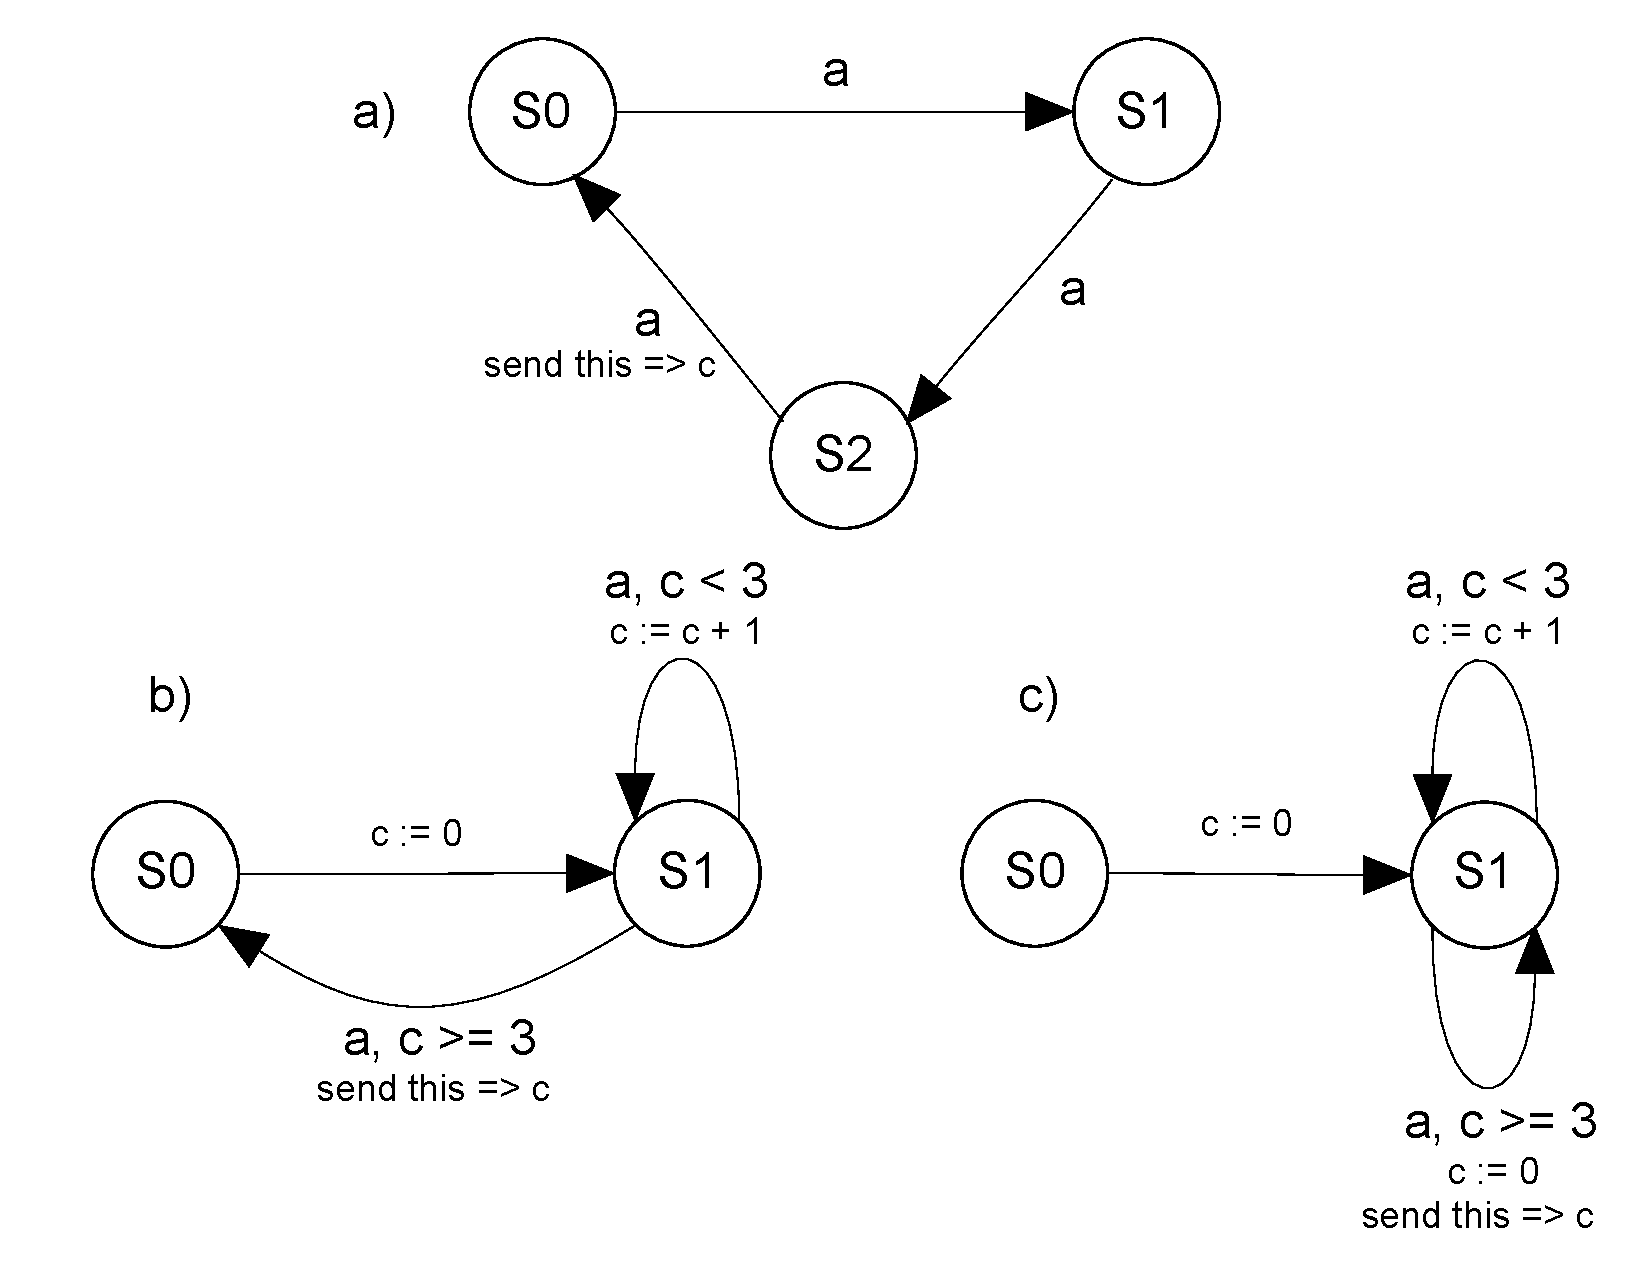
\includegraphics[scale=0.4]{figs/counter.pdf}
  \caption{The transition diagrams of the counter synchroniser.}
  \label{fig:counter}
  \end{figure}


  \item The selection predicate $\rho$

In a given state $k$ for each output channel $\omega_{m}$ we note all $i$ on which $\rho_{ki}^{m}$ is true. Those message values must be stored in a previous state and recalled in state $k$. It is expected that the boolean vector $\omega_{i} = \rho_{ki}^{m}$ has only very few true elements.

Consequently the storage mechanism that \ak\ provides for synchronisers is in the form of individual \emph{store} variables. The type of a store variable is determined when a variable is assigned.

\textbf{Example: the binary zip synchroniser}  Zip2 receives messages on its input channels and sends their concatenation to the output channel. In the resulting concatenation there's exactly one message from each input channel and those messages are ordered as they received.

The zip2 transition diagram is given in Figure \ref{fig:zip2}. The message received in the current transition is referred by a keyword \emph{this}. $ma$ and $mb$ are the store variables associated with the input channels $a$ and $b$ respectively. The statement \emph{send} indicates a sending of a message to an output channel.

  \begin{figure}[here]
  \centering
  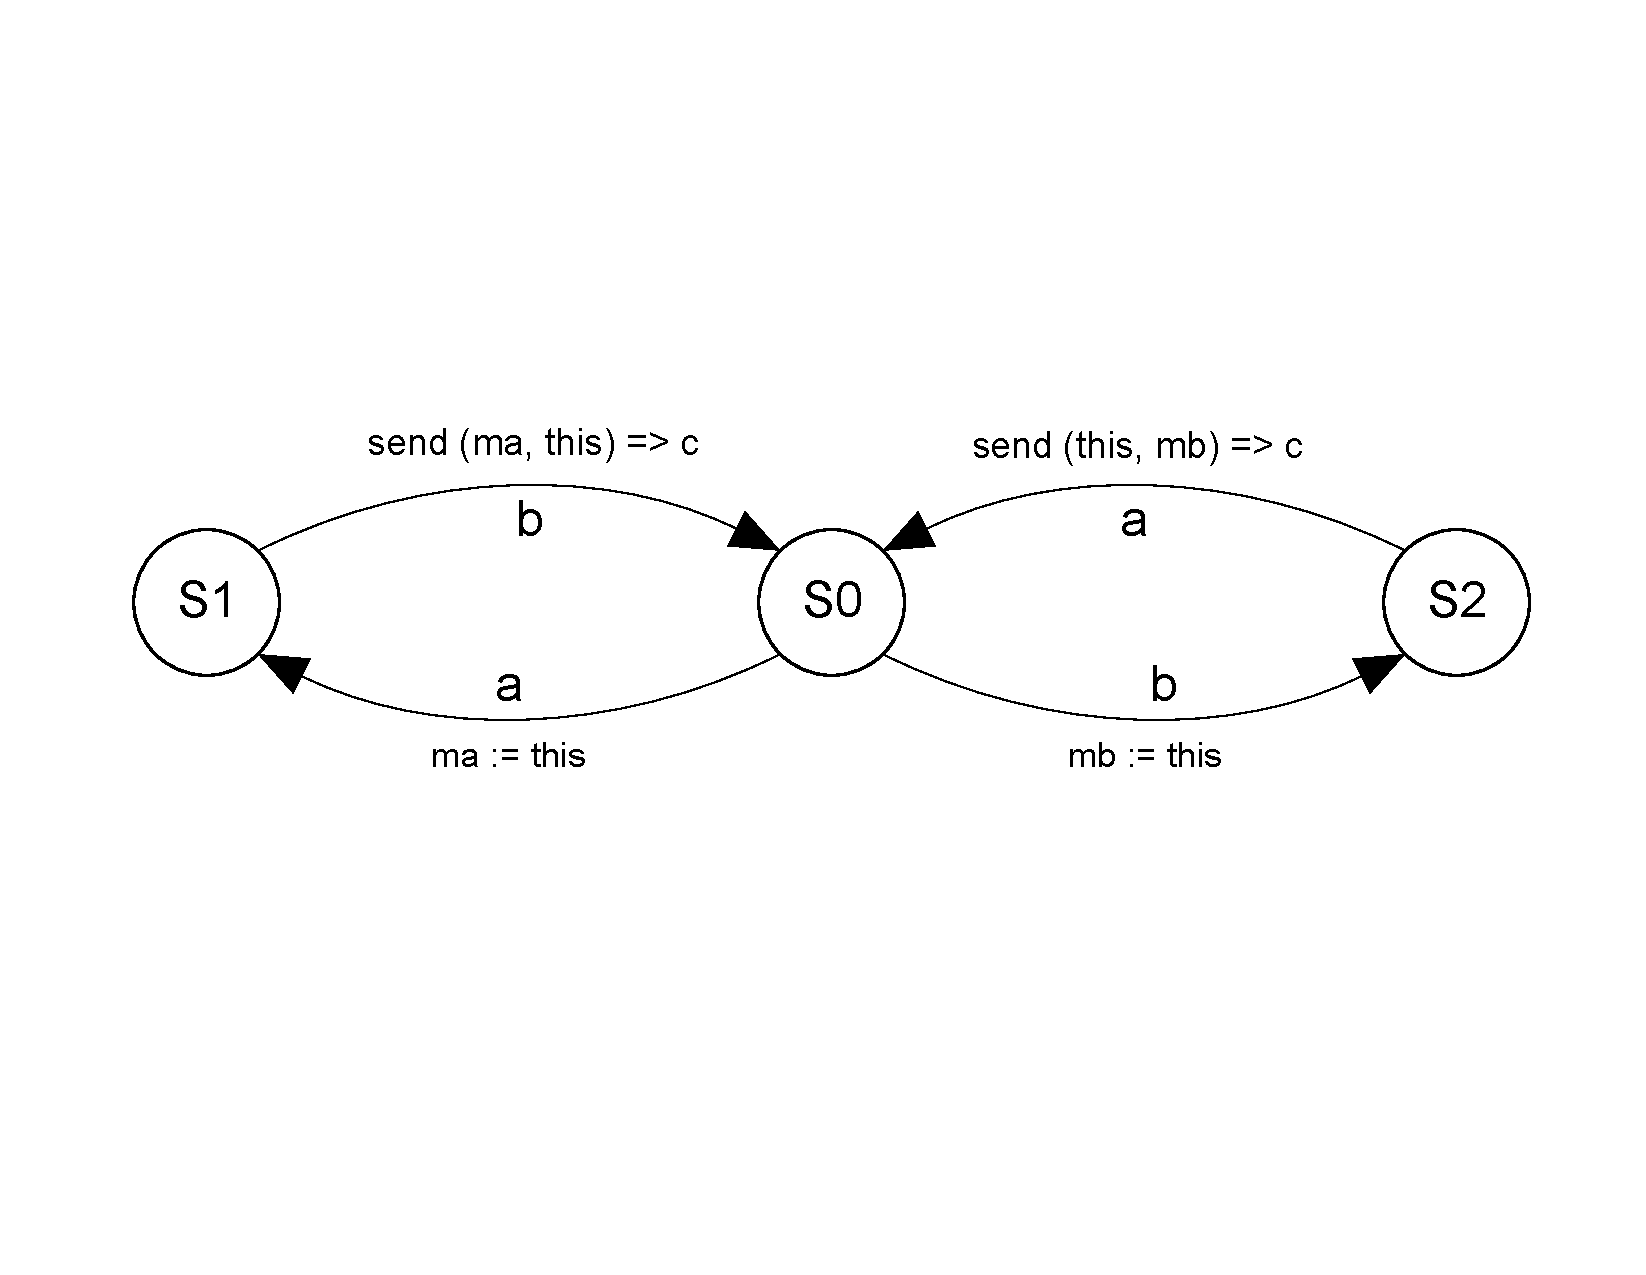
\includegraphics[scale=0.4]{figs/zip2.pdf}
  \caption{The transition diagram of the zip2 synchroniser.}
  \label{fig:zip2}
  \end{figure}

Mathematical model $S_{zip2} = (\Phi, \; \Pi)$, where
  \begin{itemize}
  \item[] $\Phi = (A, \; S, \; T)$,
    \begin{itemize}
    \item[] $C = (a, \; b)$, $P = (true)$, $A = C \times P = ((a, \; true), \: (b, \; true))$,
    \item[] $S = (s_{0}, s_{1}, s_{2})$, $s_{0}$ -- start state,
    \item[] $T$:
      \begin{tabular}{c|c|c|c}
      $A$ \textbackslash $S$ & $s_{0}$ & $s_{1}$ & $s_{2}$\\
      \hline
      $(a, \; true)$ & $s_{1}$ & $s_{1}$ & $s_{0}$\\
      \hline
      $(b, \; true)$ & $s_{2}$ & $s_{0}$ & $s_{2}$\\
      \end{tabular}
    \end{itemize}
  \item[] $\Pi \: : \: S \times \Omega \to V$,
    \begin{itemize}
    \item[] $\Omega = (c)$,
    \item[] $V = ((a, \; b), \: (b, \; a))$
    \end{itemize}
  \end{itemize}

An output message is emitted when a transition happens either from the state $s_{1}$ or the state $s_{2}$. These states are reached in two paths:
  \begin{itemize}
  \item[]
$W_{0} = ((s_{0}, \; a), \: (s_{1}, \; b))$

$\Pi \; (s_{1}, c) = \psi_{\sqcap} \; \{\mu_{0} = a \: | \: \rho_{10}^{c} \; (s_{0}) = 1, \mu_{1} = b \: | \: \rho_{11}^{c} \; (s_{1}) = 1\}$, $k = 1$, $i = 0,1$
  \item[]
$W_{1} = ((s_{0}, \; b), \: (s_{2}, \; a))$

$\Pi \; (s_{2}, c) = \psi_{\sqcap} \; \{\mu_{0} = b \: | \: \rho_{20}^{c} \; (s_{0}) = 1, \mu_{2} = a \: | \: \rho_{22}^{c} \; (s_{2}) = 1\}$, $k = 2$, $i = 0,2$ 
  \end{itemize}
  \end{enumerate}


\section{The language for \ak\ synchroniser}
We develop the language according to chosen message protocol. The protocol restricts anything but a $choice$ termed message trevelling in channels. This the syntax $on a.(x,y, ...)$ is not needed with this protocol. We may include this syntax as a syntax sugar for $uniq$ when choice has just one alternative. Originally this syntax was intended for records in channels. However, the chosen protocal doesn't allow it. For example if we want to extend the protocol for lists to travel in channels, we need to define the union of lists, possibly as a construct with 2 nested lists $(union l_1 l_2)$ and we need to extend the protocol to encode this construct. For record and choice union is easy to define. If no labels in $t_1$ and $t_2$ intersect then the resulting record of choice has all the labels from $t_1$ and $t_2$ with their values: $t = union \; t_1 \: t_2 = union \; {a:t_a} \: {b:t_b} = {a:t_a, \: b:t_b}$. When labels intersect, it is the deal for CAL solver to resolve with option to take (it should consider flow inheritance). The synchroniser just leaves it to be a union of terms:

For example for Choice: $union \; (: \: a:t_a \: :) \: (: \: a:t_b \: :) = (: \: a:union \: t_a, \: t_b \: :)$.
Same for record.


\subsection{Synchroniser code}
%% TODO fix 'channel connected to the port x' to channel x
%% Insert a footer that explains that 'channel x' is short for 'channel connected to the port x'
An \ak\ synchroniser is a finite state machine, therefore the basic building blocks of a synchroniser program are states and transitions. A state of a synchroniser is fully defined by the corresponding state of the finite state machine and the values of the state variables. A transition is the act of moving to another state which is initiated by a triggering event. A triggering event for the synchroniser transition is an arrival of a message to the associated channel. The message may be required to have a specific structure. In addition, a transition may be guarded by special conditions on the values of the state variables. If the conditions are satisfied the transition fires, otherwise it is cancelled.

Once a transition is known to fire, optional actions may be performed before the underlying state machine makes the move. These actions include changing the state and store variable values and sending messages to the output channels. In order to change the state and store variables, the synchroniser language provides state and store expressions over them.

This section gives an overview of the \ak\ synchroniser programming language. The formal grammar of the \ak\ synchroniser is provided in Appendix \ref{sync_syntax}.

  \subsubsection{Program structure}
A synchroniser program consists of a header followed by the synchroniser's body wrapped in braces. The begining of a synchroniser program is indicated by the keyword $synch$.

The header of a synchroniser program contains the synchroniser's name and the channel signature. The name is an ASCII string that follows the C convention.

The body of the synchroniser lists the state and store variables declarations and the states of the underlying finite state machine. Each state is defined by a list of transitions. Each transition lists its triggering condition which includes an optional guarding state expression, an optional list of actions, and, finally, the destination state.

%  \subsection{Macros}
%%%
%%% We removed macros from the language. The compiler must invoke a preprocessor to expand them.
%%%
%The synchroniser language provides macros to avoid having to trivially alter synchroniser programs. Macros are specified in brackets between the synchroniser's name and its channel signature. An example of a configurable synchroniser can be found in \cite{astrakahn}.

  \subsubsection{Channel signature}
The channel signature defines the input channels and the output channels of the synchroniser and their bracketing depths. The synchroniser header (Fig. \ref{min_sync_head}) declares the synchroniser $min$ with two input channels that are connected to the ports $a$, $b$ and two output channels that are connected to the ports $c$, $d$. If the bracketing depths of the channels are not specified, they are assumed to be 0. Thus, the bracketing depth of the channel $a$ is 0.

The input channel depth $-1$ indicates that the input channel is ignored in the synchroniser program. The output channel with the depth $-1$ must not have data sent to them.

\begin{figure}[h!]
\begin{lstlisting}[frame=single]
synch min (a, b:p | c:2, d:p+1)
\end{lstlisting}
\caption{The synchroniser header}
\label{min_sync_head}
\end{figure}

%% TODO remove read-only state variables

The \ak\ synchroniser allows to declare constant and configurable integer depths for the input and output channels. In addition, the depth of the output channel can be specified with an integer shift to the configurable input channel depth.

The input channels are required to have the bracketing depths specified in the signature. Thus, the channel connected to the port $a$ of the $min$ synchroniser must have zero bracketing depth. The channel connected to the port $b$ has a configurable bracketing depth $p$. Actual values of configurable bracketing depths of input channels are determined by the \ak\ compiler. %Once defined in the signature, configurable bracketing depths may be used in state expressions. They are interpreted as read-only state variables.

The output channels of a synchroniser are guaranteed to have the bracketing depths specified in the channel signature. Thus, the synchroniser $min$ must send messages to the output channel connected to the port $c$ at the depth 2 and optionally at the depths $0$, $1$. The output channel connected to the port $d$ must have the bracketing depth $p+1$ that is the depth of the input channel connected to the port $b$ shifted by $1$.


%% TODO Move all the type details to the implementation details
%% TODO The width of int type is declared explicitly to reduce the number of potential states of automata.
  \subsubsection{Variable declaration}
%% Add about state and store variables initialisation.
%% state int(8) a, b=1, c=8; // assignes a=0 b=1 c=9
%% enum (a,b,c) foo, bar=a;  // assignes foo=0 bar=a
The beginning of state variables declaration is indicated by the keyword $state$. A state variable may be either a signed integer of the constant width or a C-style enumeration. State and store variables names are user-defined indentifiers. A user-defined identifier is an ASCII string that follows the C convention.

%% TODO Should move width determining to the implementation detail
Line 1 in Fig. \ref{sync_statevar} declares state variables $a$, $b$, $c$ of width 4. Thus, all three variables are declared to have integer values in the range $[-8; 7]$. Generally, a state variable of width $n$ has integer values in the range $[-2^{n-1}; 2^{n-1}-1]$.

The state variable $foo$ that is declared in the line 2 in Fig. \ref{sync_statevar} can only be assigned the values $d$, $e$ and $f$ specified in the enumeration. The enumeration values are defined as constants if type $int$. If the values are not specified explicitly, they are assigned consequtive positive integers starting with 0. The width of the $int$ type is $\lceil \log_{2}{n} \rceil + 1$, where $n$ is the number of values in the enumeration. Thus, the variable $foo$ has integer values $d=0$, $e=1$ and $f=2$ of the width $\lceil \log_{2}{3} \rceil + 1 = 3$. If the values are specified explicitly, the width is determined as $\lceil \log_{2}{(m+1)} \rceil + 1$, where $m$ is the biggest value in the enumeration. For the variable $bar$ declared in line 3 of Fig. \ref{sync_statevar} $m=4$ and the width is $\lceil \log_{2}{(5)} \rceil + 1 = 4$.

Integer state variables and enum values can be mixed freely in state expressions. Enum values are interpreted as read-only integer state variables. % constant integers!

\begin{figure}[h!]
\lstset{numbers=left, numberstyle=\small, stepnumber=1, numbersep=8pt}
\begin{lstlisting}[frame=single]
state int(4) a, b, c;
state enum(d, e, f) foo;
state enum(x = 1, y = 2, z = 4) bar;
store msg_a, msg_b;
\end{lstlisting}
\caption{State and store variables declaration}
\label{sync_statevar}
\end{figure}

Store variables declaration begins with a keyword $store$. Line 4 in Fig. \ref{sync_statevar} declares state variables $msg\_a$ and $msg\_b$. Store variables do not need explicit type specification; their types are determined on the first assignment to the variable.

All the state and store variables are global to all the synchroniser states.


  \subsubsection{States and transitions}
States and transitions of the synchroniser define which channels are read and in what order. Fig. \ref{zip_struc} presents the code of the binary zip synchroniser's state machine. Line 1 declares the start state of the synchroniser. The $on$ clause indicates the beginning of the transitions list. In the start state the zip2 synchroniser acceptes messages from both input channels $a$ and $b$. State and store expressions associated with the transition and the destination state are specified in the braces.

\begin{figure}[h!]
\lstset{numbers=left, numberstyle=\small, stepnumber=1, numbersep=8pt}
\begin{lstlisting}[frame=single]
start {
  on:
    a { goto s1;    }
    b { goto s2;    }
}
s1 {
  on:
    b { goto start; }
}
s2 {
  on:
    a { goto start; }
}
\end{lstlisting}
\caption{State machine of the zip2 synchroniser}
\label{zip_struc}
\end{figure}

When the zip2 synchroniser is in the start state and it receives a message from the channels connected to the port $a$, the underlying state machine makes a transition to the state $s1$. In this state the synchroniser can only receive messages from channel connected to the port $b$ since there's no transition triggered by channel connected to the port $a$ and defined in this state. When the message on channel connected to the port $b$ is received, the state machine makes a transition to the start state. Lines 10-13 define similar behaviour in state $s2$.

%% Change 'scopes'. 'Blocks' probably
The synchroniser language supports top-down prioritised transition scopes. They are indicated with the $elseon$ keyword. A synchroniser in state $foo$ in Fig. \ref{sync_scope} acceptes messages from channels connected to the ports $a$, $b$, $c$ and $d$. When no destination state is specified for a transition, a synchroniser makes the transition to the current state. If all channels are ready at the same time in state $foo$, the synchroniser processes messages from either channel $a$ or $b$ first. When all messages from channels connected to the ports $a$ and $b$ are processed the synchroniser receives messages from channels connected to the port $c$. If there're no messages in channels $a$, $b$ and $c$ the synchroniser receives messages from the channel connected to the port $d$.

\begin{figure}[h!]
\lstset{numbers=left, numberstyle=\small, stepnumber=1, numbersep=8pt}
\begin{lstlisting}[frame=single]
foo {
  on:
    a { }
    b { }
  elseon:
    c { }
  elseon:
    d { }
}
\end{lstlisting}
\caption{Prioritised transition scopes}
\label{sync_scope}
\end{figure}


  \subsubsection{State expressions}
State expression is a combination of integer constants, state variables and operators, which computes and produces an integer value. The interpretation of a state expression follows C rules of precedence and association. State expressions can be assigned to state variables. In assumption that the output channel is infinite a synthetic example in Fig. \ref{sync_state_exp} counts the number of messages received from channel connected to the port $a$ between the arrivals of messages in channel connected to the port $b$. Line 1 declares the 8-bit integer $count$ and initialises it with 0. When a message from channel connected to the port $a$ is received the value of $count$ increases by 1 (line 5).

\begin{figure}[h!]
\lstset{numbers=left, numberstyle=\small, stepnumber=1, numbersep=8pt}
\begin{lstlisting}[frame=single]
state int(8) count = 0;
foo {
  on:
    a {
      set count = [count + 1];
    }
  elseon:
    b {
      set n = [count], count = [0];
      send count:[n] => c;
    }
}
\end{lstlisting}
\caption{Use of state variables and expressions}
\label{sync_state_exp}
\end{figure}

When a message from channel connected to the port $b$ is received the value of $count$ is stored in the temporary variable $n$, set to 0 and then $n$ is sent to the output channel.

The variable $n$ does not have to be declared and is considered alias for the integer expression. Temporary variables are available until the state machine of a synchroniser makes the next move.


  \subsubsection{Triggering of a transition}
The channel name on its own stands for the availability predicate for the corresponding channel, i.e. the condition that a message of any kind is available. Whether a transition takes place depends on the channel status and optionally the content of the messages.

When a message is received on a channel, it can be matched with a pattern in order to extract parameters needed to select a specific transition. Line 3 of Fig. \ref{sync_trans} checks if a message received from the input channel connected to the port $a$ contains label $x$. If it does, the contents of $x$ are stored in a temporary variable $x$. The tail of the message, i.e. everything but the part labeled $x$, is stored in a temporary variable $t$. Both $x$ and $t$ are read-only and available until the state machine makes a move.

TODO: Fix; everything in $.?v(.... \|\| tail)$ before $\|\|$ are integers.
\begin{figure}[h!]
\lstset{numbers=left, numberstyle=\small, stepnumber=1, numbersep=8pt}
\begin{lstlisting}[frame=single]
foo {
  on:
    a.(x || t)  { }
    a.?v        { }
    a.?v(x, y)  { }
    a.@[k]      { }
}
\end{lstlisting}
\caption{Message content extraction}
\label{sync_trans}
\end{figure}

To support message formats where several variants of a message are possible, a qualifier \begin{bf}?\end{bf}$\alpha$ is available as an input condition. It qualifies input messages as belonging to $\alpha$ variant. Line 4 of Fig. \ref{sync_trans} checks if a message received from channel connected to the port $a$ belongs to the variant $v$. Line 5 checks that a message that belongs to the variant $v$ contains only two records labeled $x$ and $y$. 

A channel carries a stream that consists of messages and possibly segmentation marks. In line 6 in Fig. \ref{sync_trans} a message is checked if it is a segmentation mark of the depth $k$. The depth of a segmentation mark can be a state expression.

Several different channels can be tested in any given state, however, once the readiness of a channel was established, the synchroniser is committed. Hence the set of conditions applied to the message on any input channel must be exhaustive. In Fig. \ref{sync_trans} it is not, because there no pattern for messages that do not contain label $x$, do not belong to variant $v$ and are not a segmentation mark of depth $k$ at the same time. In this case the final clause $a$\begin{bf}.else;\end{bf} is assumed. This clause discards the input message and transitions the synchroniser back to its current state.

A transition can be guarded by a state expression. In this case the transition fires only if the guarding expression evaluates to true. The synchroniser in Fig. \ref{sync_g_state_exp} sends every 256-th message to the output channel. Line 1 declares the 8-bit state variable $i$ that is initialised with 0. It is incremented every time a message from channel connected to the port $a$ is received, except when it reaches 255, in which case it is reset 0 and the received message is sent down the channel $c$. 

Values that are matched from the message can be used in guarding state expressions.
\begin{figure}[h!]
\lstset{numbers=left, numberstyle=\small, stepnumber=1, numbersep=8pt}
\begin{lstlisting}[frame=single]
state int(8) i;
start {
  on:
    a & [i < 255] {
      set i = [i + 1];
    }
    a & [i = 255] {
      set i = [0];
      send this => c;
    }
}
\end{lstlisting}
\caption{Use of guarding state expressions}
\label{sync_g_state_exp}
\end{figure}


  \subsubsection{Store expressions and sending messages}
%% TODO Probably fix it after writing about CAL terms.
Store expression is a mechanism to combine data. Data are typed in \ak\. Types are CAL terms. Store expression concatenates data in the user-defined order and therefore results in the data of a valid CAL type. The result of the store expression can be either stored in a store variable or sent down the output channel.

The example in Fig. \ref{sync_send} demonstrates the use of store expressions and the $send$ clause. In the start state the synchroniser receives messages from channel connected to the port $a$ that has label $n$ in it. In line 5 the value under label $n$ is incremented and stored in the store variable $ma$ under label $n$ together with the tail $t$. The syntactic sugar for defining a record is supported. The operator $'$ applied to the variable $x$ creates the record $'x': value(x)$.

%% TODO Provide a more convincing example for 'id and this
\begin{figure}[h!]
\lstset{numbers=left, numberstyle=\small, stepnumber=1, numbersep=8pt}
\begin{lstlisting}[frame=single]
store ma;
start {
  on:
    a.(n || t) {
      set ma = (n:[n+1] || t);
      goto s1;
    }
}
s1 {
  on:
    b {
      send ma || this => c;
      goto start;
    }
}
\end{lstlisting}
\caption{Use of store expressions and the $send$ clause}
\label{sync_send}
\end{figure}

A message received on a channel is referred to by the keyword $this$ within the active transition. In state $s1$ the synchroniser receives messages from channel connected to the port $b$. When a message is received, it is concatenated with the store variable $ma$ (line 12) and sent to the output channel connected to the port $c$.




\section{Execution order of synchroniser\label{execod}}
\begin{itemize}
\item Fairness policy
In a certain state both input channels may be ready, but a state machine receives input symbols one at a time. Which transition will be triggered under such circumstances is defined by the fairness policy: the coordinator will ensure that when more than one transition is possible in a given state, all choices will be made with the same frequency.

\item Non-deterministic $goto$

The purpose of non-deterministic gotos comes from the requirement that the synchroniser must not block the execution. If non-deterministic goto is the case then the synchroniser makes a fair transition to the state that sends messages to the channel that is not blocked.

In other words, the synchoniser avoids to make transitions to the states that send messages to blocked channels.


\item Algorithm of the execution of synchronisers
on-elseon execution order, dead $elseon$ code with $\langle chan \rangle .else$
\end{itemize}


\section{The implementation of the $aksync$ compiler}
The implementation of the compiler is written in Python (TODO: cite a cookbook), with code generation to an intermediate representation that is used by the \ak\ runtime system.

\subsection{Lexical analysis}
  \paragraph{Lexical analyser} PLY
  \paragraph{Preprocessor}
%%%
%%% We removed macros from the language. The compiler must invoke a preprocessor to expand them.
%%%
%The synchroniser language provides macros to avoid having to trivially alter synchroniser programs. Macros are specified in brackets between the synchroniser's name and its channel signature. An example of a configurable synchroniser can be found in \cite{astrakahn}.
Preprocessor performs (a C-like) macro expansion. There's no preprocessor directives in the synchroniser language (like \#define in C). Preprocessor commands are passed to it as a part of the compiler invocation command (a special flag like -Dday=night in C).

With the preprocessor we implement configuration paramenters from the original synchroniser language. Explain why they were removed. Explain what is bad about macros (can substitute anything, even a piece of code).

\subsection{Syntax analysis}
  \paragraph{Syntax alanyser} PLY. Syntax-directed translation. A translation scheme embeds program fragments called semantic actions in production bodies (TODO Dragon book, p.107)

Error handling in PLY.


  \paragraph{Abstract syntax tree} The result of syntax analysis is a representation of the source program called intermediate code. We use abstract syntax tree in the implementation.

TODO: structure of the AST.
AST generator by Eli Bendersky with the reference.

  \paragraph{Symbol table}
Symbol tables are data structures used by compilers to hold information about identifiers in a program's source code. The information is collected incrementally by the analysis phases of a compiler. Entries in the symbol table contain identifier's type, scope level, location and any other relevant information.

The role of a symbol table is to pass information from declarations to uses. A semantic action puts information about identifier $x$ into the symbol table, when the declaration of $x$ is analysed. Subsequenlty, a semantic action associated with a production that involves an identifier gets information about the identifier from the symbol table.

The scope of a declaration is the portion of a program to which the declaration applies. (TODO scope straucture of a sync program). State and store variables are visible for all transitions, therefore they belong to the global scope. State expression aliases and variables that are pattern matched belong to the local scope of a transition.

Symbol tables typically need to support multiple declarations of the same identifier within a program. We shall implement scope by setting up a separate symbol table for each scope (transition) and chaining them. The approach to the implementation of a symbol table is taken from (TODO ref Dragon book, p.89). Chaining of symbol tables results in a tree structure (probably we can simplity it somehow, because we do not really need a tree of scopes).

(TODO: probably a short description of the approach is needed. Class with fields hashtable and a link to the previous scope object, and methods 'create new', 'put', 'get' which searches the chain of tables.)

The symbol table contains types and (possibly) locations. Builing of a symbol table Dragon book p.90.

  \paragraph{Syntax-driven type inference?}
Special language constructs simplify type inference (probably it's not a good word here).

$x$ and $y$ are assigned a special type None.
\begin{figure}[h!]
\begin{lstlisting}
// typeof(x) = None means a term variable
a.?v(x, y || t) {
  // typeof(x) = None
  // typeof(y) = None
  // typeof(this) = DataTyp(h={'x': typeof(x), 'y': typeof(y)}, t='t')
  // typeof(a) = DataTyp(h={'v': typeof(this)}, t='a_tail')

  set n = [x+1], ma = (this || id:y);
  // typeof(x) = IntTyp(None)
  // typeof(n) = IntTyp(None)
  // typeof(ma) = DataTyp(h=typeof(this).h+{'id': typeof(y)}, t='t')

  send (ma || 'n':n) => c;
  // typeof(c) = DataTyp(h=typeof(ma).h+{'n': typeof(n)}, t='t')
}

a.?v(x, y || t) {
  // typeof(x) = None
  // typeof(y) = None
  // typeof(this) = DataTyp(h={'x': typeof(x), 'y': typeof(y)}, t='t')
??  // typeof(a) = DataTyp(h={'v': typeof(this)}, t='a_tail')

  set ma = (this || y);
  // typeof(n) = IntTyp(None)
  // typeof(ma) = DataTyp(h=typeof(this).h+typeof(y).h, t=tailof(this))

  send ?v(ma) => c;
  // typeof(c) = DataTyp(h={'v':typeof(ma)}, t=None)
}




// Remove variant 'v'?
a.?v(x, y || t) {
// typeof(x) = None
// typeof(y) = None
// typeof(this) = DataTyp(h={'x': typeof(x), 'y': typeof(y)}, v='v', t='t')
// typeof(a) = DataTyp(h={'v': typeof(this)}, v=None, t='tail')

set n = [x];
// typeof(x) = IntTyp(width=None)

set m = this || x || 'y || id:z
// typeof(x) = DataTyp(h={'x': None}, v=None, t=None)
// typeof(y), typeof(z) not influenced
// typeof(m) = DataTyp(h=typeof(this).h + {'x': None} + {'y': typeof(y)} + {'id': typeof(z)}, v=None, t=tailof(this))

send this || x || 'y || id:z => c
// typeof(x) = DataTyp(h={'x': None}, v=None, t=None)
// typeof(y), typeof(z) not influenced
// typeof(c) = DataTyp(h=typeof(this).h + typeof(x).h + {'y': typeof(y)} + {'id': typeof(z)}, v=None, t=tailof(this))

send ?v(this || x || 'y || id:z) => c
// typeof(c) = DataTyp(h={'v': typeof(this || x || 'y || id:z)}, v='v', t=None)

\end{lstlisting}
\label{aa}
\end{figure}

If $x$ or $y$ are used in a state expression, their type is assigned to Int.


A state expression is specified in brackets. Everything in state expression is integer.
If an assignment is being parsed and no brackets were specified in assignment expression, then it is a store expression.

  \paragraph{Static checking}
Static checks are consistency checks that are done during compilation. Not only do they assure that a program can be compiled successfully, but they also catch programming errors early. Static checking includes:
\begin{itemize}
\item Syntactic checking. Constraints such as an identifier is declared at most once in a scope (TODO: more)

Reserved words $nil$ and $this$ can't be identifiers

\item Type checking. The type rules of a language assure that an operator or function is applied to the right number and type of operands.

If an identifier was met and it is already in the current scope of symbol table, it must have the same type (int or data) as before.
\end{itemize}

    \paragraph{Tests}
Uses standard python unittest module.
Expands AST into nested list.

\subsection{Semantic analysis}
  \paragraph{Semantic analyser}
Architecture of the analyser. Pattern visitor?

  \paragraph{Checks}
\begin{enumerate}
\item Channel signature. If the output channel depth is in the form of depth expression $p+integer$, then $p$ should be the depth of one of the input channels. $p$ is not allowed anywhere in state expressions.
  \begin{itemize}
  \item (a:p | b:p+1) - allowed
  \item (a:p | b:0) - allowed
  \item (a:p | b:r) - allowed
  \item (a:p | b:r+1) - NOT allowed
  \end{itemize}
The special depth $-1$ indicated that the channel is not used. Therefore, if it is an input channel, all the transitions reading from it can be removed. If it is an output channel, and the transition that sends to this channel is valid, then an error must occur.

!!Probably avoid writing a visitor!! Visitor for ports that returns their depths which are IDs.
For the input and output channels sets that are returned by the visitor are equal.
Do we really need visitor for it?

Check that transitions in states are made on the specified in signature input channels and messages are sent on the specified output channels.

\item State variables.
State variables are in global scope.

int(n) a, b, c; n denotes only the value range of a state variable. It decreases the number of possible states of a synchroniser. $a$, $b$ and $c$ must always be within range $[0; 2^{n}-1]$ (int is unsigned). At low level state variables are machine- and target language- dependent integers.

The translation scheme in Fig. \ref{std} presents state variable types and their ranges.

(Table: grammar rule - type/width, p.375 Dragon book).
\begin{figure}[h!]
\centering
\begin{tabular}{|c|c|}
\hline
Type & Values\\
\hline
int(n) & $[0; 2^{n}-1] \cap \mathbb{Z}$\\
\hline
enum($a_1$, $a_2$, $\dots$ $a_n$) & $[0; n-1] \cap \mathbb{Z}$\\
\hline
enum($a_1=N_1$, $a_2=N_2$, $\dots$ $a_n=N_n$) & $N_1$, $N_2$, $\dots$ $N_n$\\
\hline
\end{tabular}
\caption{Computing types and their value ranges}
\label{std}
\end{figure}

(TODO: Probably it is a static check that can be done right from parser)

Check if the range condition is valid at least for assignments (int(1) x = 10 is not good, should issue a warning, check what would be assigned to x in C). For the state expressions that evaluate during the execution of the synchroniser it's probably ok to delegate the overflow checks to the C compiler.

\item State expressions. Probably it is all static check as well.
  \begin{itemize}
  \item Patterns $(x || t)$ and aliases for state expressions. $x$ and $t$ are in local scope of the active transition.

(TODO: think if it should be restricted). $x$ and $t$ musn't be declared global - otherwise it is an error??

$x$ and $t$ are read-only.

Probably should not differentiate between pattern variables and aliases. For state and store variables there's a differentiation because we need to know what is included in states of synchroniser (state vars) and what is not (store vars).

If $x$ is used in a state expression, it is integer (has the term 'number'). Tail $t$ can't be used in a state expression; $t$ is always at least a record ($t = (name: value)$).

  \item The grammar for integer expression used in our implementation of a synchroniser compiler (Appendix \ref{int_exp_gr}) is a simplified version of the C grammar for arithmetic expression.

  \end{itemize}


\item Store variables
Store variables are typed by CAL terms.
The type of a store variable is determined on the first assignment to it.

\item Store expressions
The result has a valid CAL term.
If the right-hand side of an assignment is not in brackets, it is a store expression.

\end{enumerate}


\subsection{Code optimisation}
  \paragraph{Dead code elimination}
\begin{itemize}
\item Remove unreachable states of an automaton (when there's no state variables involved).

\item Remove unreachable transitions based on Section Execution order.

\item Remove unused state, store variables and assignments (this may require some simple def-use analysis, probably can put it into symbol tables).
\end{itemize}


\subsection{Code generation}
  \paragraph{Synchroniser runtime code}
Give a class diagram?
Generator architecture - node visitor

  \paragraph{Synchroniser passport}
A synchroniser can impose some restriction on the type of messages it accepts.
In the implementation we consider that only choices travel between channels (it is unclear what is a unification of lists, how to order the elements in the resulting list).

None indicates that it is a term variable.

Input channels: Fig. \ref{a}.
\begin{figure}[h!]
\begin{lstlisting}
//term: None (term variable), Int, Record, Choice
a.(x,y||t) {
  //x - is a value not a pair. In a store expression of in a send it must be 'x
  //term(x) = None
  //term(y) = None
  //term(a) = { x:term(x), y:term(y) | $t }
  //term(this) = term(a)

  set n = [x];
  //term(x) = Int
  //term(a) = { x:term(x), y:term(y) | $t }
}

a.?v(x,y||t) {
  //term(x) = None
  //term(y) = None
  //term(this) = { x:term(x), y:term(y) | $t }
  //term(a) = (: v:term(this) | $a_t :)

  set n = [x];
  //term(x) = Int
  //term(a) = (: v:{ x:term(x), y:term(y) | $t } | $a_t :)
}
\end{lstlisting}
\label{a}
\end{figure}

Output channels: Fig. \ref{b}.
\begin{figure}[h!]
\begin{lstlisting}[frame=single]
//record union with label 'x' collision: {x:type_1, y:...} + {x:type_2, z:...} = {x:type_2, y:..., z:...}
//python's dict.update(...)
a.(x,y||t) {
  //term(x) = None
  //term(y) = None
  //term(this) = { x:term(x), y:term(y) | $t }
  //term(a) = term(this)

  set ma = (this || id:y);
  //term(ma) = term(this) || id:term(y) =
             = { x:term(x), y:term(y), id:term(y) | $t }

  send ?v(ma || n:x) => c;
  //term(c) = (: v:(term(ma) || n:x) | $c_t :) =
            = (: v:{ x:term(x), y:term(y), id:{ y:term(x) }, n:term(x) | $t } | $c_t :)
}
\end{lstlisting}
\label{b}
\end{figure}


\section{Discussion}
MDL is wider than what the presented synchroniser can synchronise. TODO: give examples. However, it need to be elaborated with the real world applications of \ak\ whether it is useful to implement it in synchronisers.

Decide how to do flow inheritance in synchronisers. This will be done outside of synchronisers. Need to somehow specify which fields are inherited and which are not. In synchroniser transitions we can pick fields of an accepted message, with ehich we want to do something in synchroniser. However, there may be many fields in the message and some of them do not need to be inherited. In theory we could pick all the fields that we want to inherit along with the fields we want to work with, and them concat them and send them to then output channel. But there may be too many to specify manually for eack transition in the synchroniser caused by the channel.

% TODO change this uglyness
\chapter{The Serial Replication in \ak\ }
%The serial replication combinator implements recursive computations and the loop construct with pipeline parallelism.
In this chapter we explain the machinery behind the serial replication in \ak\ and the role of synchronisers in it. We introduce the concept of the forward fixed point for the replication pipeline and show how it is used to organise the output from the infinite chain of replicas. In order to supress the growth of the replicas chain, we present the concept of the reverse fixed point and show how it is used to optimise some replicas in the head of the chain.


%TODO
%First of all, the semantics of AstraKahn on the TPL is described in terms of structures put in place for the coordinator, i.e. a controlling agent, or indeed a group of agents, responsible for progress and communication of the KPN vertices.
%


    \section{\ak\ Approach to the Serial Replication}
The serial replication combinator creates conceptually infinite number of copies of its operand network, and connects them in a chain. Replication is demand-driven, hence replicas are created dynamically in runtime. A fresh replica is \emph{inactive}\footnote{More generally, we call a replica inactive when all of its synchronisers are in their start states, none of its channels has messages in them and no box is running}, hence it does not necessarily require significant resouces since \ak\ boxes are stateless and synchronisers require no resouces in their start state\footnote{When a synchroniser transitions back to the start state, it flushes its store variables}. Indeed the cost of replication is only felt when the replicas are active, which is the case when the first message is received until all messages have left the replica and all its synchronisers have returned to their start states.

In S-Net, the output from the replication pipeline is based on the record subtyping in the type system. The replication combinators in S-Net require the programmer to specify a termination pattern, so that each record that is a subtype of this pattern leaves the replication pipeline throught the output stream.

In \ak\, the output from the replication pipeline is inspired by the concept of a fixed point. From the mathematical point of view a fixed point of a function is an element of the function's domain the function maps to itself. That is to say, the function $f(x): X \to Y$ has a fixed point in $x_0 \in X$ iff $f(x_0) = x_0$. The definition yields an important termination consideration
\begin{equation}
\exists n: \; \forall k<n \;\; f^{(k)}(x) \neq f^{(n)}(x) \; \land \; \forall k \ge n \;\; f^{(k)}(x) = f^{(n)}(x) \nonumber
\end{equation}
when the function $f$ is computed recursively\footnote{$f^{(n)}(x)$ denotes $\underbrace{f(f(\dots f}_n (x) \dots))$}. The serial replication combinator implements such a computation as shown in Fig. \ref{fig:fp}. After the $n$-th replica has processed the message $f^{(n-1)}(x) \neq x_0$ the computation reaches the fixed point $x_0$, and the message $x_0$ is sent on to the output channel of the serial replication network $f^{*}$.
\begin{figure}[h!]
\centering
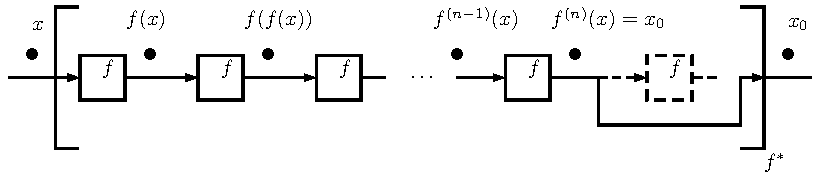
\includegraphics[scale=0.8]{figs/chapter_03_fp.pdf}
\caption{The recursive computation in \ak\ }
\label{fig:fp}
\end{figure}

The number of iterations $n$ needed to reach the fixed point is not known in advance, meaning that in order to utilize the fixed point as shown in Fig. \ref{fig:fp}, \ak\ must be able to detect the fixed point message right at the time it is produced by the $(n-1)$-th replica. Therefore, just like in S-Net, \ak\ needs to be provided with a pattern that matches all the fixed point messages of the operand network. In S-Net, the serial replication combinator requires to specify the pattern as one of its operands, while in \ak\ the pattern can be encoded within the operand network due to the ability of synchronisers to check the message content and perform different actions depending on the result of the check. The pattern is extracted from the operand network due to the fact \ak\ can analyse synchronisers.
%Due to separation of concerns \ak\ does not have to analyse the box code\footnote{except for CAL passport generation}, therefore the fixed point must be defined in synchronisers or the network topology of a net.

The chain of replicas grows as the computation progresses, however, in the example in Fig. \ref{fig:fp} the computation is carried out only by a single replica in the tail of the chain. The replicas in the head of the chain have processed the message and are not used anymore. In order to suppress the growth of the chain, \ak\ is committed to detect such replicas and optimise the connection by removing them. Since \ak\ boxes are stateless, an operand network can have a state that is fully defined by the states of its synchronisers. A replica of the operand network can be removed from the chain safely iff the replica is in a state, in which it transmits any message without change, i.e. any message it receives is a fixed point. We will call such a state of the replica the reverse fixed point state.

In the remainder of the chapter we give formal definitions for a fixed point message and reverse fixed point state and provide algorithms for the \ak\ compiler to detect them. Consequently we will call the fixed point message the forward fixed point.
%The intention of the forward fixed point is to cut an infinite tail of replicas chain. The reverse fixed point is an optimisation of an input connection that suppresses the growth of the replicas chain. 


    \section{Forward Fixed Point}
%We will now explain how the pattern to match the fixed point messages can be encoded within the operand network.
Once the computation in the serial replication network has reached the fixed point, newly created replicas are known to transmit the fixed point messages without change. \ak\ does not analyse boxes\footnote{Except for the CAL passport generation}, so it can conclude about the operand network behaviour only from its synchronisers. Thus, in order for the operand network to be analysable by \ak\ for the required behaviour, it must contain a path that does not traverse boxes and may traverse synchronisers. Because a newly created replica is inactive and hence the synchronisers in it are in their start states, the start states of the synchronisers that belong to the path must have a special transition that would implement sending of the message on to the next synchroniser along the path. Since transitions can be conditional on the message content, the fixed point pattern, or rather the fixed point condition, can be encoded in these special transitions.

%1) synchronisers approach (only detects integer fields like S-Net)
The existence of a forward fixed point requires the operand network to have some topological properties that are formally defined as follows. Consider a network $N$ that has an input and an output channel, both named $x$.

\begin{definition}\label{ffp_def}The network $N$ is said to have a forward fixed point in $x$ if and only if the following requirements are satisfied:
\begin{enumerate}
\item There exists a condition $P(m)$ on the content of the message $m$ received by the network on the input channel $x$ under which it follows a unique non-branching path to the output channel $x$ without traversing any boxes
\item The path can traverse synchronisers, but then whenever $P(m)$ is true and the synchroniser is in the start state, it must accept $m$ and transition back to the start state while sending the message $m$ on the path unchanged and without producing any other output%TODO fix
\end{enumerate}
\end{definition}

The condition $P$ may not be unique for each network, and when it is not, the fixed point condition of the network is a disjunction of all such conditions. The condition can also be a tautology, in which case the forward fixed point is called unconditional. When the path traverses a single synchroniser, the fixed point condition is defined exclusively by the synchroniser transitions that loop around the start state and send on the accepted messages unchanged. When the path traverses several synchronisers, the fixed point condition of the network is a conjunction of the fixed point conditions of these synchronisers. We demonstrate the construction of the fixed point condition with the example operand network $N$ pictured in Fig. \ref{fig:ffp}.

\begin{figure}[h!]
\centering
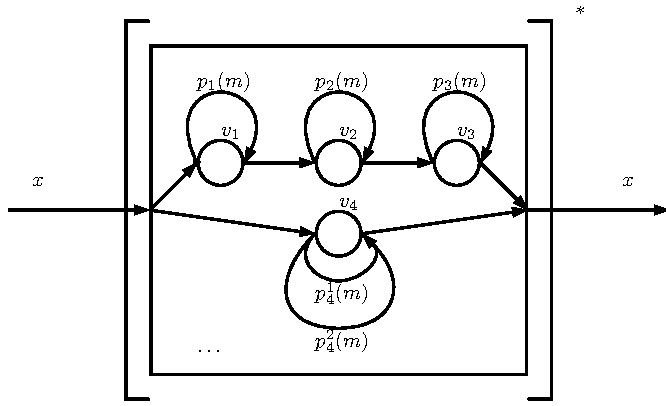
\includegraphics[scale=0.8]{figs/chapter_04_ffp.pdf}
\caption{Forming of the forward fixed point condition of a network}
\label{fig:ffp}
\end{figure}

Apart from all the paths that traverse boxes, the operand network $N$ has a unique path $[s_1, \: s_2, \: s_3]$ that traverses only synchronisers. The synchroniser $s_2$ has two transitions that loop around the start state and send on messages they accept unchanged with the firing conditions $p^{1}_2(m)$ and $p^{1}_2(m)$. A message $m$ is a fixed point for the network $N$ when it satisties any of these conditions, i.e. $p^{1}_2(m) \lor p^{1}_2(m)$. The synchronisers $s_1$ and $s_3$ have fixed point conditions $p_1(m)$ and $p_3(m)$ respectively, where $p_i(m) = p^{1}_i(m) \lor \dots p^{j}_i$, $i=1,3$ and $j$ is the number of transitions in each synchroniser that loop around the start state and send on messages unchanged. Then the fixed point condition of the network $N$ is $p_1(m) \land (p^{1}_2(m) \lor p^{1}_2(m)) \land p_3(m)$.

The definition \ref{ffp_def} requires the synchronisers that traverse the fixed point path to transition back to the start state when the fixed point message was sent on. This restriction can be relaxed, however, in this case for each synchroniser the programmer would have to maintain a transition that checks for the fixed point condition in every state of the synchroniser.


    \subsubsection{Output from the Serial Replication Network}
Now we will clarify how the serial replication network is wired to the rest of the \ak\ application network and how the output is produced.

Strictly speaking, the serial replication is not just a wiring pattern since it does not simply wire the replicas of its operand network. It also creates a set of output channels and augments the replicas with some auxiliary synchronisers.
%However, in the main it wires the replicas in a serian fashion and we will consequently call the FPS a connection.

%We denote the FPS connection as $A^{*} = A' \: .. \: A' \: .. \: A' \: .. \: \dots$, where $A'$ is the network that contains $A$ and provides additional wiring to ensure that all output channels of $A'$ match its input channels bijectively.

The serial replication $N^{*}$ defines the output channel set $\mathcal{N}_{out}$ as follows:
\begin{equation}
\mathcal{N}_{out} = \{ name(c) \: | \: c \in \mathcal{O} \land fp(c) \}\nonumber
\end{equation}
where $\mathcal{O}$ is the output channel set of $N$ and the predicate $fp(c)$ is true on any channel $c$ that has a forward fixed point. The serial replication creates a set of fresh output channels $\mathcal{O}^{*}$ taking the names from the set $\mathcal{N}_{out}$. A message that comes to an inactive replica on any channel $c$ with $name(c) \in \mathcal{N}_{out}$ and satisfies the fixed point condition on that channel is immediately transferred to the identically named output channel from $\mathcal{O}^{*}$. A network in Fig. \ref{fig:ffp_out} demonstrates how the output is produced from the serial replication of a network that has a single input and a single output channel.

\begin{figure}[h!]
\centering
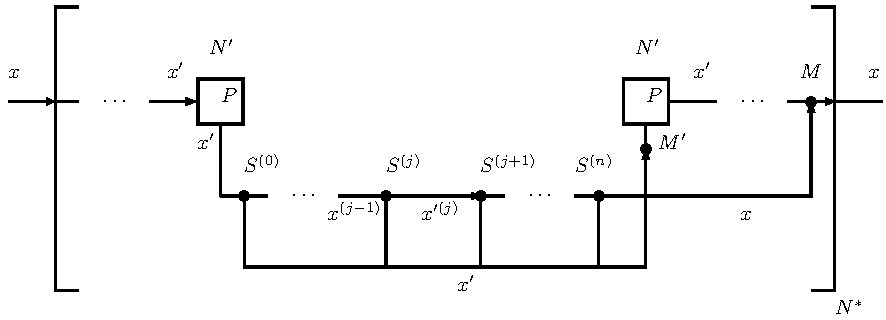
\includegraphics[scale=0.8]{figs/chapter_04_ffp_out.pdf}
\caption{Output from the serial replication network}
\label{fig:ffp_out}
\end{figure}

The operand network $N$ has the fixed point condition $P = \underset{j}{\bigcap} \; p_j$, where $p_j$ is the fixed point condition extracted from the $j$-th synchroniser ($1 \leq j \leq n$) on the fixed point path of $N$. In order to check whether a message $m$ in channel $x'$ satisfies the condition $p_j$, a synchroniser $S^{(j)}$ is inserted in front of every inactive replica $N'$. If $p_{j}(m)$ is true, the synchroniser sends the message $m$ on to the input channel of the next synchroniser $S^{(j+1)}$ to check whether $p_{j+1}$ is satisfied. Otherwise, the message $m$ is sent to the input channel $x'$ of the next replica of $N$. The listing of the synchroniser $S^{(j)}$ is given in Fig. \ref{ffp:synch_filt}. We shall note that $\forall j \;:\; p_j = \underset{j,k}{\bigcup} \: p^{(k)}_j$ the synchroniser $S^{(j)}$ has $k$ transitions that implement checking of the atomic conditions $p^{(k)}_j$.
\begin{figure}[h!]
\begin{lstlisting}[frame=single,mathescape]
synch $S^{(j)}$ ($x'^{(j-1)}$ | $x'^{(j)}$, $x'$)
{
  start {
    on:
      $x'^{(j-1)}$.$p_j$ {
        send this => $x'^{(j)}$;
      }
      $x$.else {
        send this => $x'$;
      }
  }
}
\end{lstlisting}
\caption{The synchroniser $S^{(j)}$}
\label{ffp:synch_filt}
\end{figure}

The merger $M'$ gathers messages that do not satisty the fixed point condition from all synchronisers $S^{(j)}$ between two consequtive replicas on $N$ and resends them to the input channel of the next replica. The merger $M$ gathers message that satisfy the fixed point condition and resends the messages to the output channel $x$ of the serial replication network $N^{*}$.

%An FPS is a form of replication wiring whereby an infinite chain of replicas is created, connected in series. The connection is denoted as A* for any operand network A and can be thought of as the equivalent of $A^{*} = A'..A'..A'.. \dots$ where $A'$, called the streamlining of the vertex A, is a network that contains A and provides some additional wiring to ensure that each output channel of A? matches an input channel and vice versa. We will dwell on the streamlining procedure a little further down, and at this point only remark that if all output channels of A match its input channels bijectively, A' = A.

    \subsection{Forward Fixed Point Detection}
%    \subsubsection{The Fixed Point Path Search}
%Algorithm that uses extract_ffp, returns the list of all atomic FP conditions for the fixed point message
The existence of a forward fixed point requires the synchronisers that are traversed by the fixed point path to have at least one transition in their start states that accepts the fixed point messages and send them on unchanged and without producing any other output. Coded in the synchroniser language, the transition that defines the fixed point condition $p$ in channel $x$ is presented in \ref{ffp:synch_fp}.
\begin{figure}[h!]
\begin{lstlisting}[frame=single,mathescape]
start {
  on:
    x.$p$ {
      send this => x;
    }
  ...
}
\end{lstlisting}
\caption{The start state of a synchroniser that encodes the fixed point condition $p$ in channel $x$}
\label{ffp:synch_fp}
\end{figure}

We shall note, that there exists no more transition on the channel from the start state with the same structure (a single \emph{send} clause). Otherwise, the synchroniser has the fixed point condition that is a disjunction of conditions in such transitions. The algorithm in Fig. \ref{fig:ffp_extract} checks if a forward fixed point exists in channel $x$ and extracts the fixed point condition from the synchroniser source code. The algorithm supports the renaming of channel $x$ in the synchroniser. Moreover, it may be the case that the transitions that cause a fixed point in the synchronisers send messages to different output channels. The algorithm detects such a situation, however, the branching of the fixed point path is resolved in the context of the whole network.

\begin{figure}[h!]
\noindent\fbox{%
\begin{minipage}{\dimexpr\linewidth-2\fboxsep-2\fboxrule\relax}
\begin{algorithmic}[1]
\Require the abstract syntax tree of the synchroniser program ($synch$), the input label of a channel to test for a forward fixed point ($x$)
\Ensure a dictionary $(a, CondList)$, where $a$ is the output label of the fixed point channel and $CondList$ is the list of atomic fixed point conditions

\Statex
\Function{extract\_ffp}{$synch, x$}
  \State $state\gets get the start state tree from synch$

  \State $CondDict\gets nil$
  \Statex
  \For{\textbf{each} \emph{trans in trans\_list}($state$)}
    \If{$get\_port$($trans$) $\neq x$}
      \State \textbf{continue}\Comment{\emph{the transition reads from another channel}}
    \EndIf
    \If{$get\_goto$($trans$) $\neq$ (\tangled{start} $\lor$ $\emptyset$)}
      \State \textbf{continue}\Comment{\emph{the transition does not loop around the state state}}
    \EndIf
    \If{$get\_assign$($trans$) $\neq$ $\emptyset$}
      \State \textbf{continue}
    \EndIf
    
    \State $send\gets get\_send$($trans$)
%    \If{$get\_port$($send$) $\neq$ \tangled{x}}
%      \State \textbf{continue}\Comment{\emph{messages are sent to another channel}}
%    \EndIf 
    \If{$get\_msg$($send$) $\neq$ $this$}
      \State \textbf{continue}
    \EndIf

    \State $cond\gets get\_condition$($trans$)
    \If{$cond$ \emph{is not CondDataMsg} $\lor$ $cond$ \emph{is not CondEmpty}}
      \State \textbf{continue}\Comment{\emph{the condition cannot be a segmentation mark or an} \texttt{.else}}
    \EndIf

    \State $out\_port\gets get\_port$($send$)
    \If{$cond \in CondDict$($out\_port$)}
      \State $CondDict$($out\_port$)$\gets CondDict$($out\_port$) \texttt{..} $cond$
    \Else
      \State $CondDict\gets CondDict$ \texttt{..} ($out\_port$, [$cond$])
    \EndIf

  \EndFor

  \Statex
%  \If{$|keys$($CondDict$)$| \neq 1$}\Comment{\emph{if the number of entries in the dictionary is not 1}}
%    \State \emph{error}
%  \EndIf

%  \If{$CondDict = nil$}
%    \State \emph{error}\Comment{\emph{the synchroniser does not have the fixed point}}
%  \EndIf

  \State \textbf{return} $CondDict$
\EndFunction
\end{algorithmic}
\end{minipage}%
}
\caption{Extracting the fixed point condition from a synchroniser (assumes that channel $x$ is declared as an input and an output channel of the synchroniser)\label{fig:ffp_extract}}
\end{figure}

The fixed point condition of an \ak\ network is formed by the fixed point conditions of its synchronisers that are traversed by the fixed point path. Networks in \ak\ are represented as graphs, thus the fixed point detection is a graph search problem.

A network graph is a directed multigraph because in \ak\ two nodes are not restricted to be connected with more than one edge. The graph has four types of nodes, namely a box, a synchroniser, a merger and a network. The fixed point path may traverse nodes of any type except for boxes. If the path traverses a node that is a network, the network must have a forward fixed point as well.

The fixed point detection algorithm (Fig. \ref{fig:ffp_detect}) is based on the depth-first search algorithm with the following considerations:
\begin{itemize}
\item The first and the last node of the fixed point path for a particular input channel are known, thus, only the paths between these two nodes in the graph are traversed

\item If the search encounters a box, the traversed path is rejected

\item If the search encounters a synchroniser, the fixed point condition of the synchroniser is extracted using the function $extract\_ffp$ in Fig. \ref{fig:ffp_extract}. If the synchroniser has no fixed point condition, the traversed path is rejected. Otherwise, the search continues only for the successors of the node that were detected by $extract\_ffp$

\item If the search encounters a merger, it immediately continues with its only successor

\item If the search encounters a node that encapsulates a network, the fixed point detection is run on the network. If no fixed point path exists for the network, the traversed path is rejected.
\end{itemize}

The fixed point detection algorithm runs only on acyclic networks. The wrap-around wiring makes \ak\ networks cyclic, however, the wrap-around channels cannot carry a fixed point. Therefore, these channels must be filtered before the fixed point detection is run.


%\begin{figure}[h!]
%\noindent\fbox{%
%\begin{minipage}{\dimexpr\linewidth-2\fboxsep-2\fboxrule\relax}
%\begin{algorithmic}[1]
%
%\Require an operand network ($net$), a channel to test for a forward fixed point ($x$)
%\Ensure a set of fixed point conditions on the channel
%
%\Statex
%
%\Function{detect\_ffp}{$net, x$}
%  \State $start\gets$\emph{get a node that has an input port x}
%  \State $end\gets$\emph{get a node that has an output port x}
%  \Statex
%
%  \State \textbf{return} $get\_cond\_list$($net, x, start, end$)\Comment{\emph{Fig. \ref{fig:ffp_get_cond}}}
%%  \If{$|Lists| \neq 1$}
%%    \State \textbf{return} \emph{error}
%%  \EndIf
%%  \State \textbf{return} $Lists$
%\EndFunction
%\end{algorithmic}
%\end{minipage}%
%}
%\caption{A forward fixed point detection in channel $x$ (assumes the network graph is connected)\label{fig:ffp_detect}}
%\end{figure}


\begin{figure}%[h!]
\noindent\fbox{%
\begin{minipage}{\dimexpr\linewidth-2\fboxsep-2\fboxrule\relax}
\begin{algorithmic}[1]
\Require an operand network graph ($graph$), a channel to test for a forward foxed point ($x$), the first and the last node in the fixed point path ($start$, $end$), the list of fixed point conditions gathered along the path ($cond\_list$, optional with the default value $empty\_list$)

\Ensure a set of fixed point conditions on the channel
\Statex

\Function{detect\_ffp}{$graph$, $x$, $start$, $end$, $cond\_list=empty\_list$}
  \If{$start$ \emph{is a box}}
    \State \textbf{return} $empty\_list$
  \EndIf
  \Statex

  \If{$start$ \emph{is a synchroniser}}
    \State $CondDict\gets extract\_ffp$($start, x$)
    %What if there're few synch paths and the synch does not have the fixed point???
    \If{$CondDict = nil$}
      \State \textbf{return} $empty\_list$
    \EndIf

    \State $Lists\gets empty\_list$

    \State $cond\_list\gets cond\_list$ \textbf{..} $start\_cond$ %add check if cond already exists in cond_list

    \For{\textbf{each} \emph{succ\_node in succ\_nodes}($start$)}
      \State $out\_port\gets get\_label$($edge$($start, succ\_node$))
      \If{$out\_port \in keys$($CondDict$)}
        \If{$start = end$}
          \State \textbf{return} $cond\_list$
        \EndIf

        \State $NewLists\gets detect\_ffp$($graph, out\_port, succ\_node, end, cond\_list$)

        \For{\emph{new\_list in NewLists}}
          \State $Lists\gets Lists$ \textbf{..} $new\_list$\Comment{\emph{the fixed point path branches if $|Lists|>1$ }}
        \EndFor

      \EndIf
    \EndFor

    \State \textbf{return} $Lists$
  \EndIf
  \Statex

  \If{$start$ \emph{is a merger}}
    \If{$start = end$}
      \State \textbf{return} $cond\_list$
    \EndIf
    \State $out\_port\gets get\_out\_port$($start$)\Comment{a merger has a single output port}
    \State $succ\_node\gets get\_succ\_node$($start$)
    \State \textbf{return} $detect\_ffp$($graph, out\_port, succ\_node, end, cond\_list$)
  \EndIf
  \Statex

% It does not work for 2 consecutive nets in the path
  \If{$start$ \emph{is a network}}
    \State $start\gets$\emph{get a node that has an input port x}
    %run detection for every node that has no successors, must be one path in total
    %\State $end\gets$\emph{get a node that has an output port x} %not x, the channel is unknown

    \State $Lists\gets detect\_ffp$($graph, x, start, end$) %it can be empty_list as well if the network does not have a fixed point, then the path is rejected
    \If{$start = end$}
      
      \State \textbf{return} $cond\_list$ \textbf{..} $Lists$

    \EndIf
    \State \textbf{return} $Lists$
  \EndIf

\EndFunction
\end{algorithmic}
\end{minipage}%
}
\caption{A forward fixed point detection in channel $x$ (assumes the network graph is connected)\label{fig:ffp_detect}}
\end{figure}



    \subsection{Discussion}
The approach we have presented relies on the ability of synchronisers to encode some checks of the message content and perform different actions depending on the result of a check. Since synchronisers can only check values of record fields that are known to be integers, the approach is not applicable for iterative computation with the floating-point precision. %However, to the best of our knowledge this is in accordance with S-Net, where the fixed point matching pattern
To enable this class of algorithms, in addition to the synchroniser-based approach we provide a fixed point detection strategy 
%
%
%only detects integer fields like S-Net)
%2) wire-through (applicable to detect non-integer fixed points, for iterative computation with the floating-point presicion)
%
%%%%%%%%%
%In \ak\, a message leaves the replication pipeline exclusively via a special complement channel that is wired to the rest of the \ak\ network. The programmer has to make sure that the messages to be sent on are detected within the operand network and sent to this channel. 
%
%Thus, the serial replication in \ak\ enforces a topological property of the operand network that is formally defined as follows. Consider the serial replication $N^{*}$ of an operand network $N$ with the input and output channel sets $\mathcal{I}$ and $\mathcal{O}$ respectively. Consequently, the set of matched inputs and outputs is $\mathcal{M}(\mathcal{I}, \: \mathcal{O}) = \mathcal{I} \cap \mathcal{O}$. In order for the serial replication $N^{*}$ to be able to produce output to the channel $x \in \mathcal{M}(\mathcal{I}, \: \mathcal{O})$, at least one box or a synchroniser in $N$ must have the output port wired to the complement channel $x'$. The \ak\ compiler recognizes the use of complement channels and checks whether the operand network topology has this property. If it does not, the compiler reports an error and aborts the compilation.
%
%The \ak\ runtime is committed to support the dynamic rewiring for complement channels. The serial replication implementation depends on the \ak\ runtime implementation, particularly the primitives the runtime system provides for the network construction. We briefly describe two approaches to the serial replication implementation with respect to the available primitives.
%%%%%%%%%
%
that relies on a special port wiring primitive $P$ that transmits messages immediately from one port to another without storing them. The programmer now has to make sure that the fixed point messages are detected within the operand network\footnote{It can be done in a box} and sent to $P$. The messages cascade through all the active replicas via a chain of $P$ wires and leave the replication network when they encounter an inactive replica. The example in Fig. \ref{fig:ffp_new} demonstrates how the approach works.

The operand network $A$ in Fig. \ref{fig:ffp_new} has a single input port $x$ and two output ports. The output port $x$ is intended for the messages that proceed to the the next replica of $A$ in the chain, and the output port $x'$ is a complement port for the messages that are supposed to leave the replication pipeline. The serial replication network $A^{*}$ has a single input and a single output port both named $x$. During the compilation, the operand network $A$ is encapsulated into the special network $N$ it as shown in Fig. \ref{fig:ffp_new}. The network $N$ inherits all the ports from $A$ and adds a corresponding input port $x'$. The input and output ports $x'$ of $N$ are connected with the wiring primitive $P$. The output and the input ports $x'$ of the consequent replicas of $N$ are connected with the wiring primitive $P$ as well.
\begin{figure}[h!]
\centering
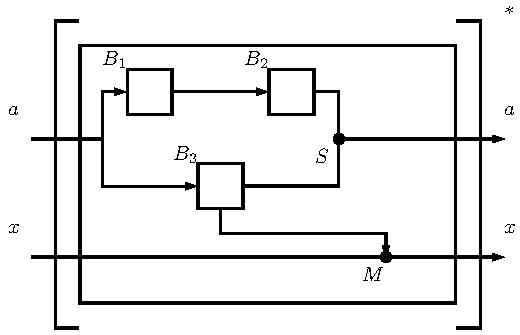
\includegraphics[scale=0.8]{figs/chapter_04_ffp_new.pdf}
\caption{The operand network $A$ (top) and a possible implementation of its serial replication $A^{*}$ (bottom)}
\label{fig:ffp_new}
\end{figure}
A message that $A$ sends to the output port $x'$ cascades through all the active replicas. Once it has reached an inactive replica, the output channel $x$ of $A^{*}$ is dynamically wired to the output port $x'$ of the last active replica of $N$. When an inactive replica becomes active, the port $x'$ is rewired with the input port of this replica using $P$.



%The second approach to the serial replication implementation relies on a merger with variable number of inputs. When a replica of $A$ sends a message to the output port $x'$, a new input channel is created for the merger $M$ and wired to the output port $x'$ of the replica as shown in Fig. \ref{fig:ffp_new_1}. The merger's output port is wired to the output channel $x$ of $A^{*}$.
%\begin{figure}[h]
%\centering
%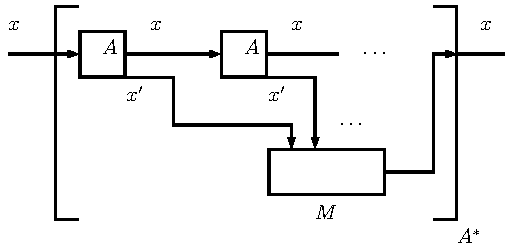
\includegraphics[scale=0.8]{figs/chapter_04_ffp_new_1.pdf}
%\caption{Another possible implementation of the serial replication $A^{*}$}
%\label{fig:ffp_new_1}
%\end{figure}
%
%%The serial replication implements a loop with variable tripcount



    \section{Reverse Fixed Point\label{rfp}}
% TODO: I don't like the reason. Why was the reverse fixed point introduced?
% reverse fixed point is the basic optimisation that preserves growth of the replicas chain.
As the chain of replicas evolves, it may be the case that some replicas in the head of the chain are active yet they just transmit messages without a change. \ak\ is commited to detect such replicas and optimise the connection so that the data are sent directly to a replica that is ready to process it. 

In this section we provide the approach to the reverse fixed point.

Consider a vertex $v$ that has an input and an output channel, both named $x$.

\begin{definition} The vertex $v$ is said to have a reverse fixed point in $x$ if and only if the following statements hold:

\begin{enumerate}
\item A unique non-branching path from the input to the output channel $x$ exists that does not traverse any boxes.

\item Every synchroniser $S_i$ on the path has a subset of states, which we denote as $s_i$, such that in each of these states every message on the path is immediately transferred without being changed or even stored, causing the synchroniser to remain in the same state\footnote{It should also be borne in mind that the values of any state variables form a part of the synchroniser state}. In a state from $s_i$ the synchroniser $S_i$ may still be sensitive to other input channels, as long as this does not, under any circumstances, cause a transition to a state outside $s_i$.
\end{enumerate}
\end{definition}

The vertex $v$ is said to be in a reverse fixed point state on channel $x$ when each $S_i$ is in a state that belongs to its $s_i$.

%%%%%%%%%
%%  Motivation for the reverse fixpoint
%%%%%%%%%
The reverse fix-point is defined to unify backslash \ combinatior and the star in terms of their functionality, which was never done in S-Net(TODO which patterns??). The intention is that they only differ in the pressure propagation strategy. The backslash creates no pressure (TODO why??) in its looped channel, and the start mantains and propagates the pressure in channels between instanses.

% probably a picture
%
% backslash (* is the synchroniser)
%      _________
%    \|/ _____  |
% ____*_|     |_|
%       |_____|
%
%
% Star with the reverse fix point
%        __________________
%      _|___________       |
%    _|______       |      |
%   |    __ \|/ __ \|/ __ \|/ __
% --*---|__|-*-|__|-*-|__|-*-|__|-- ...
%

The reverse fix point is more the way to write code. It is the way to program a loop dependency, when the result of the iteration depends not only on the result of the previous iteration but on the new incoming data. The difference with backslash is in the pressure propagation.

If you want the feature, you must define a closed set of translating states in every synchroniser on the fp path.


    \subsubsection{Rewiring of the Reverse FPS}
The reverse fixed point optimises an input connection that has to cascade through the chain to a replica that is ready to accept the data. Any input channel $x$ wired to an active replica $A_i$ that transitions to a reverse fixed point state on that channel is disconnected from $A_i$ and dynamically rewired to the input channel $x$ of the next replica on the chain $A'_{i+1}$.

%pic



%\section{Fixed Point Detection Algorithms}
%
%    \subsection{Forward Fixed Point Detection\label{ffp_detect}}
%The approch we proposed in section \ref{approach} makes the forward fixed-point detection trivial. The forward fixed-point detection does not require synchroniser analysis anymore. The \ak\ compiler just checks that the forward fixed-point exists in the network topology.
%
%We split the forward fixed-point detection problem into the following subproblems:
%\begin{itemize}
%\item Choose a data structure to represent a net
%\item Provide an algoritm for the fixed-point path detection
%\item Provide an algoritm for recursive fixed-point check
%\end{itemize}
%
%% Provide detection algorithm
%
%\ak\ compiler needs to just detect the forward fixpoint from the network topology (answer 'yes' or 'no' if the fixpoint exists). If the fixpoint was not found then the network is infinite and inconsistent.
%
%Forward fixpoint detection is pure network topology analysis. Find a way in a net graph that goes exclusively through mergers and some other vertex output to this channel.
%

    \subsection{Reverse Fixed Point Detection\label{rfp_detect}}
%%% Synch state conditions for the reverse fixpoint state
A message is not changed by the synchroniser in some state when:
- message is sent out by the synchroniser without any changes and storing in any transition including user-specified $else$ ($this$)

A message sent in autogenerated $else$ transition is disregarded by the synchroniser.

If a message is sent out in a user-defined $else$ then we have to make sure that the message get to this $else$. Before $else$ the channel may be tested for variants and segmantation marks, so we have to make sure that the message doesn't contain these variants/not a segmentation mark whatever.
%%%%%%


Choose any convenient structure for nets to resolve fix points. It may be a kind of graph that traversing it it's easy to find paths that only consist of synchronisers.
It could be a hypergraph (each vertex may have several inputs and several outputs) with type vertices (something that indicates whether vertex is a synchroniser or a box)

This chosen structure can be build in the net parser of from the net compiler internal data structure.

Then we need to represent a set of possible paths in this hypergraph that only contain synchronisers. And a traversal of the hypergraph to find all these paths.

Then we analyse every synchroniser in each path for the satisfiability of fix point conditions.


    \subsection{Discussion}
%channels are ordered, need to insert synchronisers
Order of messages in the reverse fixed point may be changed, because a message may put the replica into the reverse fixed-point state and go for processing into this replica. In this case the messages that came to the replica that is in the reverse fixed-point state may overcome the message processed in the replica. This changes the order of messages. If the progrmmer wants to preserve the order, he must mind it. It may be fixed by creating a separate channel for RFP messages and putting a synchroniser that blockes the RFP channel while there's no message from the output channel (this is for operand network with one input channel, with two it can be more dificult if there're races between the channels that wire replicas).

The replication combinator is just a wiring pattern that does not have to guarantee race-safety. For example, if the operand network is not race-safe, the star is not race-safe as well.


\chapter{Towards statistical properties of synchronisers}
Brief explanation of the role of synchronisers in learning for proliferation (that initial throughput value estimation is needed as well as initial channel sizes)

How did we come to the idea of using a statistical model?
What is a statistical model in general? (See wiki page) How are they used?
The practical side of statistical model: The model of the relatioships between various object parameters
 
In absence of environment for experiments and example applications artificial load is used.

%Практический смысл статистической модели:
%1) Характеристики $T'_{i}, \; j'_{i}$ являются начальными значениями для алгоритма пролиферации
%2) Начальные размеры каналов

\section{Statistical model}
Let $S = (\Phi, \; \Pi)$, where $\Phi = (A \subseteq C \times P, \; S, \; T)$, $\Pi \: : \: S \times \Omega \to V$ be a synchroniser with $|C| = m$ input channels, $|\Omega| = n$ output channels and the transtion matrix $T$. All channels $c_{i}, \: i = 1,m$ and $\omega_{i}, \: i=1,n$ are finite FIFO-queues that have lengths $L^{(in)}_{i}, \: i = 1,m$ and $L^{(out)}_{i}, \: i=1,n$ as shown in Fig. \ref{fig:stat_mod}.

% Inkscape figure
  \begin{figure}[h] %here!
  \scalebox{0.8}{
    \includesvg{figs/stat_mod}
  }
  \caption{A statistical model of a synchroniser}
  \label{fig:stat_mod}
  \end{figure}

%Explaining basic structure of channel and input channel producer properties
Every input channel $c_{i}, \; i = 1,m$ is connected to a producer $P_{i}$ that sends to this channel on average of $T_{i}$ messages per unit time with an independent jitter (i.e. standard deviation) $j_{i}$. $T_{i}$ may also be interpreted as the throughtput of the $i$-th producer. The output parameters of the synchroniser $T_{i}$ and $j_{i}, \; i=1,n$ assume that the channel $c_{i}$ has infinite length.

%Explaining synchroniser consuming characteristics
When messages are placed on a synchroniser's input queue they may or may not be consumed immediately. In some states the synchroniser may block the input channel. Let $T'_{i}, \: i=1,m$ be the average number of messages accepted by the synchroniser per unit time and $j'_{i}$ the standard deviation of $T'_{i}$.

%Synchroniser producing characteristics
A synchroniser is the producer for its output queues $\omega_{i}, \: i=1,n$. Let $T'_{i}, \: i=1,n$ be the average number of messages sent by the synchroniser to the output channel $\omega_{i}$ per unit time and $j'_{i}$, again, the standard deviation of $T'_{i}$.

%Ouptut channels consumers
The synchroniser's output channels are connected to processes $C_{i}, \: i=1,n$ that consume messages from these channels. Let $T_{i}, \: i=1,n$ be the average number of messages consumed by the process $C_{i}$ per unit time and $j'_{i}$ the standard deviation of $T_{i}$.

%problem statement
\begin{problem}Find relations between $(T_{i}, \: j_{i})$, $(T'_{i}, \: j'_{i}), \: i=1,m+n$, $L^{in}_{i}, \: i=1,m$ and $L^{out}_{i}, \: i=1,m$.
\end{problem}

%From statistics point of view
The model can be constructed in a different way. We focus on the interarrival time of messages instead of the throughput of the components. The interarrival time $t_{i}, \: i=1,m+n$ of messages in the channel $c_{i} \cup \omega_{i}$ is a random variable distributed according to a continuous two-parameter probability density function $p_{i} \: (t < t_{i}) = p_{i} \: (\mu_{i}, \sigma^2_{i}, t_{i})$, where $\mu_{i} = E[t_{i}]$ is the expectancy and $\sigma^2_{i} = Var[t_{i}]$ is the variance of $t_{i}$.

%%
%% TODO Draw a picture:
%%             t_i
%%        *-----------*
%%  ------*-----------*--------> t
%%        i          i+1
%%

If the interarrival time $t$ has the PDF $p_{t}(t)$ then the throughput $T = \frac{1}{t}$ has the PDF $p_{\frac{1}{t}}(t)$ that is inverse to $p_{t}(t)$. An inverse distribution is obtained by applying the transformation theorem (TODO: reference a good book) to $p(t)$. The transformation theorem states that for a continuous random variable $X$ with the PDF $p_{X} (x)$ and a function $g$ that is monotonous on its domain of definition the random variable $Y = g(X)$ has the PDF $p_{Y} (x) = |\frac{d}{dx}g^{-1}(x)|\cdot p_{X} (g^{-1}(x))$, where $g^{-1}(x)$ is the inverse function for $g(x)$ and $\frac{d}{dx}g^{-1}(x)$ is its derivative. Applying the theorem for the interarrival time $t \sim p_{t}(t)$ and the throughtput $T = g(t) = \frac{1}{t} \sim p_{\frac{1}{t}}(t)$ we get
\begin{IEEEeqnarray}{rCl}
g^{-1}(t) &=& (\frac{1}{t})^{-1} = \frac{1}{t}\nonumber\\
p_{\frac{1}{t}}(t) &=& |\frac{d}{dt}(\frac{1}{t})| \cdot p_{t}(\frac{1}{t}) = \frac{1}{t^2} \cdot p_{t}(\frac{1}{t})\nonumber
\end{IEEEeqnarray}
Knowing $p_{\frac{1}{t}}(t)$ the expectancy and the variance of the throughtput $T$ are obtained from the standard formulae
\begin{IEEEeqnarray}{rCl}
E[T] &=& \int_{0}^{\infty} t \cdot p_{\frac{1}{t}} (t) dt = \int_{0}^{\infty}\frac{1}{t} \cdot p_{t}(\frac{1}{t}) dt\nonumber\\
Var[T] &=& \int_{0}^{\infty} t^2 \cdot p_{\frac{1}{t}} (t) dt = \int_{0}^{\infty}p_{t}(\frac{1}{t}) dt\nonumber
\end{IEEEeqnarray}

\section{I don't know how to name it}
When all the time $T_{i} > T'_{i}$, $i=1,m$ then it doesn't matter what is the length of the input queue $L^{(in)_{i}}$ it will always be full. The same is with the output queues of the synchroniser: when $T'_{i} > T_{i}$, $i=1,n$ the output queue $L^{(out)}_{i}$, $i=1,n$ will always be full. Therefore, we are only interested in cases where $T_{i} = T'_{i}$, $i=1,m+n$. We are seeking for the queue lengths $L_{i} = L_{i} (T_{i}=T'_{i}, j_{i}, j'_{i})$, so that anytime the number of messages in the queue would be $l_{i} < L_{i}$. In other words, we are seeking for the queue length $L_{i}$ that minimizes the probability of messages loss for given jitters $j_{i}$ and $j'_{i}$ and rate $T_{i} = T'_{i}$.

We have 3 parts to analyse in the system:
\begin{enumerate}
\item The producer $P_{i}$, $i=1,m$ send out messages into the output channel with the rate $T_{i}$ and the jitter $j_{i}$ in assumption the output channels have infinite length. The synchroniser connected to this channels then consumes the messages with the rate $T'_{i} = T'_{i} (T_{i}, TD)$. When the length of the channel $L_{i}$ is finite and one the jitters $j_{i}$ and $j'_{i}$ is too big the channels may sometimes get full. The producer is suspended when it output channels are full, thus the full channel affects $T_{i}$ and $j_{i}$ of the producer.

\item The influence of $TD$ on the syncroniser's output rates. Messages arrive to the synchroniser's input channels with the rates $T_{i}$ and jitters $j_{i}$, $i=1,m$. Find the output rates $T'_{i} = T'_{i} (T_{i}, TD)$ and jitters $j'_{i} = j'_{i} (j_{i}, TD)$, $i=1,n$ in assumption that the input and the output channels are infinite.

Assume the synchroniser produces one message in the $i$-th output channel immediately when it has $(N_1, N_2, \dots N_m)$ messages in its input channels $(c_1, c_2, \dots c_m)$. The the arrival of the message to the $i$-th output channels happens the most often when $E[N_1 \cdot c_1] = E[N_2 \cdot c_2] = \dots = E[N_m \cdot c_m]$ and $Var[N_1 \cdot c_1, N_2 \cdot c_2, \dots N_m \cdot c_m]$ is minimal. $N_i \cdot c_i$, $i=1,m$ here denotes the event of arrival of $N_i$-th message in the channel.

For a Poisson process $Pois(\lambda)$ the arrival of the $n$-th message is distributed according to the Erlang distribution $Erlang(n, \lambda)$ with the expectancy $\frac{n}{\lambda}$ and the variance $\frac{n}{\lambda^2}$.

Draw graphs for the pure zip2 throughput(variance) with infinite queue lengts for Poisson processes and for inverse gamma processes. Probably draw a graph for the less trivial synchroniser, for ex. (a,2b)->c.

\end{enumerate}

We have to somehow find the balance equations for the synchroniser to consider it all.


Proliferation: combining and splitting Poisson processes


\textbf{Some obvious properties of the model}
Let $l_{i}, \; i = 1,n$ be the actual number of messages stored in any moment of time in channels $L_{i}$. Then the following is true:
  \begin{itemize}
  \item If anytime $l_{i} < L_{i}$, then $T'_{i} = T_{i}$, $i = 1,m$;
  \item If sometime $l_{i} = L_{i}$, then $T'_{i} < T_{i}$, $i = 1,m$;
  \item If $l_{i} > 0$, then $T'_{i} = T_{i}$, $i = m+1,n$;
  \item If $l_{i} = 0$, then $T'_{i} < T_{i}$, $i = m+1,n$.
  \end{itemize}


\section{The plan of study}
%TODO: These all need better explanation w.r.t (Some obvious properties of the model)
%Influence of finite input channel lengths on producers


$T_{i}$ and $j_{i}, \; i=1,m$ are the characteristics of producers in assumption that the channels $c_{i}, \; i=1,m$ they are connected to, are infinite. A finite channel length affects these values. If a channel is full, messages can't be placed in it anymore, so $T_{i}$ decreases. (TODO: what happens to $j_{i}$, does it decrease as well?)

%Synchroniser input characteristics
The affected values $T_{i}, \; j_{i}, \; i=1,m$ change $T'_{i}, \; j'_{i}$. Also $T'_{i}$ and $j'_{i}$ are affected by the transition diagram of a synchroniser causing input channel blockings.

%Influence of finite output channel lengths on synchroniser
If output channels of a synchroniser have finite lengths, it affects the output characteristics of a synchroniser $T'_{i}$ and $j'_{i}, \; i=m+1,n$ as finite input channels lengths affect producers.

%Influence on synchroniser consumers
The characteristics of synchroniser consumers are not affected directily by finite channels lengths. They are directly affected by $T'_{i}$ and $j'_{i}, \; i=m+1,n$.


%The plan of study
%What kind of synchronisers is studied
In this project we study only synchronisers whose transition diagrams have deterministic transitions, i.e a transition diagram doesn't depend on message content. If more that one transition possible at the same time, than all choices are made with the same frequency.

%Describe the idea for a study. We have 3 problems with a synchroniser: input channels are finite, transition diagram is random (fixed by the language), output channels are finite. Decribe the order in which these problems are studied (the strategy).

We break down the problem into parts:
  \begin{enumerate}
  \item Study the part of a system that doesn't depend on the output channels
    \begin{itemize}
    \item Find $T'_{i}$ and $j'_{i}, \; i=1,m$ depending on $T_{i}, \; j_{i}, \; i=1,m$ and finite channel lengths $L_{i}, \; i=1,m$;
    \item Investigate how $T_{i}, \; j_{i}, \; i=1,m$ are affected by $L_{i}, \; i=1,m$;
  \end{itemize}

  \item Study the part of a system that depends on the output channels
    \begin{itemize}
    \item Find "ideal" $T'_{i}$ and $j'_{i}, \; i=m+1,n$ with assumption that output channels have infinite lengths;
    \item Study an impact of finite output channels on $T'_{i}$ and $j'_{i}, \; i=m+1,n$;
    \item Investigate how $T_{i}$ and $j_{i}, \; i=m+1,n$ of consumers are affected.
    \end{itemize}
  \end{enumerate}


Stability condition $\frac{\lambda_{arr}}{\lambda_{dep}} < 1$.
\section{Relevant work}


Queueing theory, queueing networks with blocking
-Poisson
-Non-poisson
Production systems perfomance


\section{Modeling a system}

  \subsection{Modeling channels}
Channels act as FIFO-queues. Message arrivals in a channel are independent events with interarrival time $\Delta t$ distributed according to the gamma distribution: $\Delta t \sim Gamma (k, \theta, t)$. Gamma distribution is chosen because of two reasons:
    \begin{itemize}
    \item it is a well-studied distribution that generates positive values, i.e. its domain of definition is $t \in [0;\infty]$, and interarrival times must be positive,
    \item it is closed to the convolution operation if the parameter $\theta$ is fixed: $Gamma_(k_{1}, \theta) * Gamma (k_{2}, \theta) = Gamma (k_{1} + k_{2}, \theta)$; this property helps to significantly simplify heavy computations involving convolutions.
    \end{itemize}

According to the central limit theorem, any distribution could be chosen -- it should not change results significantly. (Explain why?)

TODO Put a graph somewhere with the number of messages in a channel over time (the channel is finite and connected to a synchroniser) Probably appendix with the Brownian motion

  \subsection{Modeling artificial load}
Describe the modeling of a synchroniser with a general case transition diagram (data structures, algorithms, tools, etc)
    \begin{itemize}
    \item For the unlimited queue
    \item For the limited queue
    \end{itemize}

  \subsection{Limitations of the model}
Describe the limitations of this model (only considers choosing a transition by choice frequency if more than one channel are ready)


\section{Application of Markov chains to synchronisers}
In this section we explain how to find $T'_{i}$ and $j'_{i}, \; i=1,n$ using discrete-time Markov chains.
  \subsection{Introduction to discrete-time Markov chains}
A short introduction to discrete-time Markov networks.

The states and the transition probability matrix $P$. The transition probabilities do not depend on how the state was reached. The matrix $P$ has the following properties: the sum of all elements in each raw is 1, and $lim_{n - \infty} P = P_{steady}$. The elements in each column of the matrix $P_{steady}$ have the same value and the sum of elements in (each) raw is 1. These probabilities are called steady state probabilities.

  \subsection{Structure of a chain}
\textbf{States} States of a chain describe all the possible states of input channels. By a state of a channel at time $t$ we assume the number of messages stored in it at time $t$. If a synchroniser has $A^1, \; A^2, \; \cdots A^m$ input channels, then the states of a corresponding chain are $A^1_{l_1} A^2_{l_2} \cdots A^m_{l_m}$, where $l_i, \; i=1,m$ is the number of messages in the channel $A^i$ at any time $t$.

    Provide a sketch of the algorithm to find the states. The algorithm is recursive. We have the reduced set of events that corresponds to time $t$ we chose. Then we put each event of the set to the synchroniser and record the state of queues. We run this procedure for each new state we get until we get a new state. This algoritm stops because the queues, the set of events and the set of states of he synchroniser are all finite.


\textbf{Transitions}
A transition is any tuple of messages we may get in the channels during time $t$. Defining a transition like this we state that any state is reachable from any state with just one step (need a proof?).
However, making a transition $(a^1,a^1)$ from the state $A^1_{l_1=1} A^2_{l_2}$ in the system where $|A^1|=2$ produces a lost message on the channel $A^1$. To consider lost messages we modify the state adding the number of lost messages to it: $A^1_{l_1} L^1_{k_1} A^2_{l_2} L^2_{k_2}$.

For example, take an abstract system having 2 input channels of length $l>2$. Assume the system is in such state when the chain is in state $A^1_0 A^2_0$ and the channel $A^2$ is blocked. During some time $t$ we may get any number of messages in the input channels. We consider transitions where we get 0 or 1 messages in each input channel $A^i, \; i={1;2}$. The interarrival time in both channels is Gamma-distributed with parameters $k=2$ and $\theta=0.5$: $t \sim Gamma \: (t,\theta)$. Then the probability to have one message in a channel is $p = p\:(t) = Gamma \:(k,\theta,t)$. The probability to have one message in a channel and not to have a message in another channel $P_{1,0} \: (t) P_{0,1} \: (t) = p(1-p)$. The probability to have messages in both channels $P_{1,1} = p^2$.

(A graph showing $p_{1,0}(t)$ and $p_{1,1}(t)$)

Whe can chose $t$ so that many transitions are cut off because their probability is very small.



A transition from the state $A^1_{l^1_1} A^2_{l^1_2} \cdots A^m_{l^1_m}$ to the state $A^1_{l^2_1} A^2_{l^2_2} \cdots A^m_{l^2_m}$ when we get $(l^2_1-l^1_1)$ messages in $A^1$, $(l^2_2-l^1_2)$ messages in $A^2$, \dots and $(l^2_m-l^1_m)$ messages in $A^m$. Because state machine recieves one symbol at time, there will be $\sum_{i=1}^{m}{(l^2_i-l^1_i)}$ transitions made in total.


Let $L_i, \; i=1,m$ be the length of the channel $A^i$. Obviously, $l_i <= L_i, i=1,m$. The number of states in the chain is


Describe what are the states of the chain ($A_{i} B_{j} L_{k}$). How the number of states depends on the length of the channels. Why number of states is unlimited (because of $L_{k}$).

Example: zip2
  \subsection{Approximation}
Markov chains only can be used when the arrival process is memoryless (a Markov process). In our system the arrival processes are not Markov, however we can try to approximate the model with the Markov model of higher order.

Why can we assume that the arrival processes are independent? They all come from the same source.

-discrete time
-events in channels

Describe the continous case first. Show that why the discretisation is reasonable.
Describe the discrete case. How $L_{k}$ is cut (by choosing possible events $(n,a,b,ab,...)$)

How we chose the set of possible events. We want the most minimal set possible that shows the dependence of steady-state probabilities on the distribution parametes.

%TODO: Come up with a good name for it
  \subsection{How to find $T'$ and $j'$}
dT = $\frac{sum of steady-state probabilities where messages are lost)}{t_{t}}$

%or subsection?
\section{Good-enough channel length?}
$l \sim \frac{Dk}{\langle k \rangle}$, where $Dk = \sum_{k} (k - \langle k \rangle)^{2} a_{k}$, $\langle k \rangle = \sum_{k} k a_{k}$.


\section{Example: application of the Markov chain to the zip2 synchroniser}
  \subsection{Modeling the throughput}
$T = T \: (\sigma, l)$, where $\sigma = \sigma_{a} = \sigma_{b}$ - variance in both channels, $l = l_{a} = l_{b}$ - length of both channels. See \ref{fig:t_s}
    \begin{figure}[here]
    \centering
    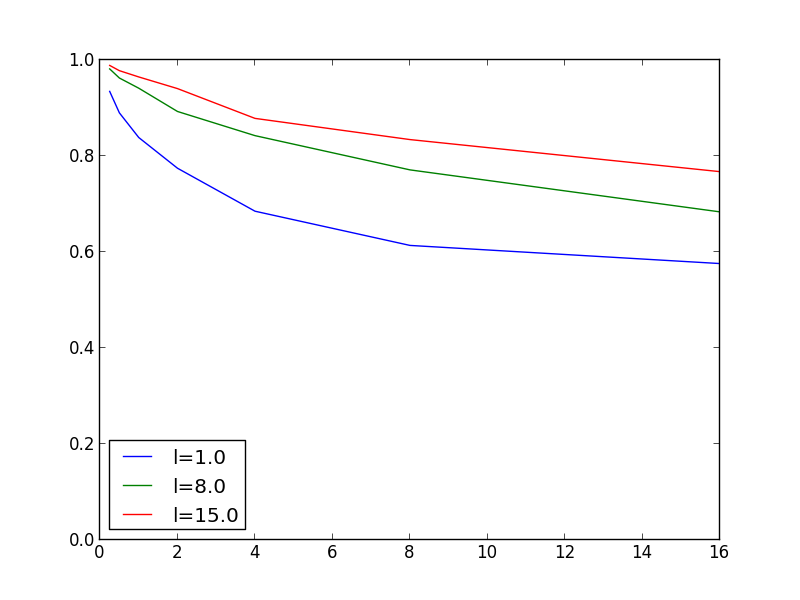
\includegraphics[scale=0.4]{figs/thr_(disp,l).png}
    \caption{$T = T \: (\sigma, l)$.}
    \label{fig:t_s}
    \end{figure}

Explain the shape of the graph when $\mu \sim \sigma$ or $\mu >> \sigma$.
Plot a graph for $0 < \sigma < \frac{\mu}{2}$.

  \subsection{Analytical results}
-States of the chain
Why we do not consider lost messages separately for each channels in the case of zip2. 

-events in channel (the minimal set for the zip2 synchroniser)
First, we try the most minimalistic set $(n,a,b)$. Let $F_{a}(t) = Gamma(k, \theta, t)$ the distribution of interarrival times in the channels. Then the probability of one message $a$ coming to the channel $A$ in time $t_{t}$ $P_{a} = F_{a}(t_{t}) = Gamma(t_{t})$. The same is for a message $b$ coming to the channel $B$ in time $t_{t}$: $P_{b} = F_{b}(t_{t}) = Gamma(t_{t})$. Note that the discretion time $t_{t}$ must be chosen so that the ptobability os an event $ab$ in time $t_{t}$ is almost zero: $P_{ab}(t_{t}) = convolution! Gamma(t_{t})^2$. The probability to see the event $a$ arrived in $A$, channel $B$ is empty $P_{a} = Gamma(t_{t})(1-Gamma(t_{t})) = Gamma(t_{t}) - Gamma(t_{t})^2 \sim Gamma(t_{t})$. The probability to see the event $n$ (nothing arrived) in the channels over time $t_{t}$ $P_{n} = (1-p)^2 = 1 - 2 Gamma(t_{t}) + Gamma(t_{t})^2 \sim 1 - 2 Gamma(t_{t})$. The total probability of all possible events in the system $P_{n} + P_{a} + P_{b} = 1 - 2 Gamma(t_{t}) + Gamma(t_{t}) + Gamma(t_{t}) = 1$ as it should be. Then we fill the Markov transition probabilities matrix $P$ for the system's states and solve the matrix equation $xP = x$. Then we find that steady-state probabilities do not depend on the parameters of the distribution in the channels which means that we should consider more events.

Then we take the set of events $(n,a,b,ab)$, for which $P_{a} = P_{b} = Gamma(t_{t})(1 - Gamma(t_{t}))$, $P_{ab} = Gamma(t_{t})^2$ and $P_{n} = (1 - Gamma(t_{t}))^2$. For this set we see the dependence of the steady-state probabilities on $Gamma(t_{t})$.

-time $t_t$
If we expect just one message to come to a channel, then we may take the expected mean of the distribution as the discretion time $t_{t} \sim m(Gamma(k,\theta)) = k \theta$.


Build $P_{steady}$, solve $x P_{steady} = x$, dT = $\frac{\sum{x_l}}{t_t}$, $T' = T - dT$.

Expand $T'$ for $\sigma << \mu$. Plot two graphs on the same picture.



\bibliographystyle{unsrt}
\bibliography{report}


\begin{appendices}
%%
%%  APPENDICES FOR THE CHAPTER 2
%%
\chapter{The syntax of the \ak\ syncroniser}

  \section{The full grammar\label{sync_syntax}}
\setlength{\grammarindent}{8em} % increase separation between LHS/RHS
\begin{figure}[h!]
\scriptsize
\begin{grammar}
<sync> ::= `synch' <ID> `(' <input> [`,' <input>]* `|' <output> [`,' <output>]* `)' \\
           `{' <decl>* <state>$^+$ `}'

<input>  ::= <ID> [`:' (<ID> | <NUMBER>)]

<output>  ::= <ID> [`:' <depth\_exp>]

<depth\_exp> ::= <ID> | <NUMBER> | <ID> `+' <NUMBER> | <ID> `-' <NUMBER>

<decl> ::= `store' <id\_list> `;'
        \alt `state' <type> <id\_list> `;'

<type> ::= `int' `(' <NUMBER> `)'
                  \alt `enum' `(' <id_list> `)'

<state> ::= <ID> `{' `on:' <trans\_stmt>$^+$ [`elseon:' <trans\_stmt>$^+$]* `}'

<trans\_stmt> ::= <ID> [`.' <condition>] [`&' <int\_exp> ] <actions>

<condition> ::= `@' <ID>
             \alt `?' <ID>
             \alt [`?' <ID>] `(' <id_list> [`||' <ID> ]`)'
             \alt `else'

<actions> ::= `{' [<set\_stmt>] [<send\_stmt>] [<goto\_stmt>] `}'

<set\_stmt> ::= `set' <assign> [`,' <assign>]* `;'

<assign> ::= <ID> `=' (<int\_exp> | <data\_exp>)

<send\_stmt> ::= `send' <dispatch> [`,' <dispatch>]*  `;'

<dispatch> ::= <msg\_exp> `=>' <ID>

<msg\_exp> ::= `@' <ID>
           \alt `@' <int\_exp>
           \alt [`?' <ID>] <data\_exp>
           \alt `nil'

<data\_exp> ::= <data>
             \alt `(' <data> `)'

<data> ::= <item> [`||' <item>]*

<item> ::= `this'
        \alt <ID>
        \alt `\'' <ID>
        \alt <ID> `:' <rhs>

<rhs> ::= <int\_exp>
          \alt <ID>

<goto\_stmt> ::= `goto' <id\_list> `;'

<id\_list> ::= <ID> [`,' <ID>]*

<int\_exp> ::= `[' <int_exp_c> `]'
\end{grammar}
\caption{The syntax of the \ak\ synchroniser}
\end{figure}


    \section{The integer expression grammar\label{int_exp_gr}}


    \section{Keywords, reserved words and punctuation\label{sync_kw}}
The keywords, the reserved words and the punctuation used in the \ak\ synchroniser syntax are given in Fig. \ref{sync_kw}.
\begin{figure}[h!]
\centering
\begin{tabular}{|c|p{0.7\textwidth}|}
\hline
Keywords & synch, store, state, int, enum, start, on, elseon, else, do, send, goto\\
\hline
Reserved words & nil, this\\
\hline
Punctuation & braces, brackets, parantheses, the comma, the dot, the semicolon, the plus sign, the minus sign, the ampersand, the at sign, the question mark, the bar-bar sign, the equality sign, the arrow\\
\hline
\end{tabular}
\caption{\ak\ synchroniser keywords, reserved words and punctiation}
\end{figure}

%%
%%  APPENDICES FOR THE CHAPTER 2
%%
\chapter{Some effects for the zip2 synchroniser}
  \section{One of the channels queues is always empty}
TODO

  \section{Brownian motion in unlimited queues}
Explain why the phenomena is observed for $\langle (n_{a} - n_{b})^{2} \rangle$. Explain the similarity of fluctuations of $n_{a} - n_{b}$ the the Brownian motion.
  \begin{figure}[h!]
  \centering
  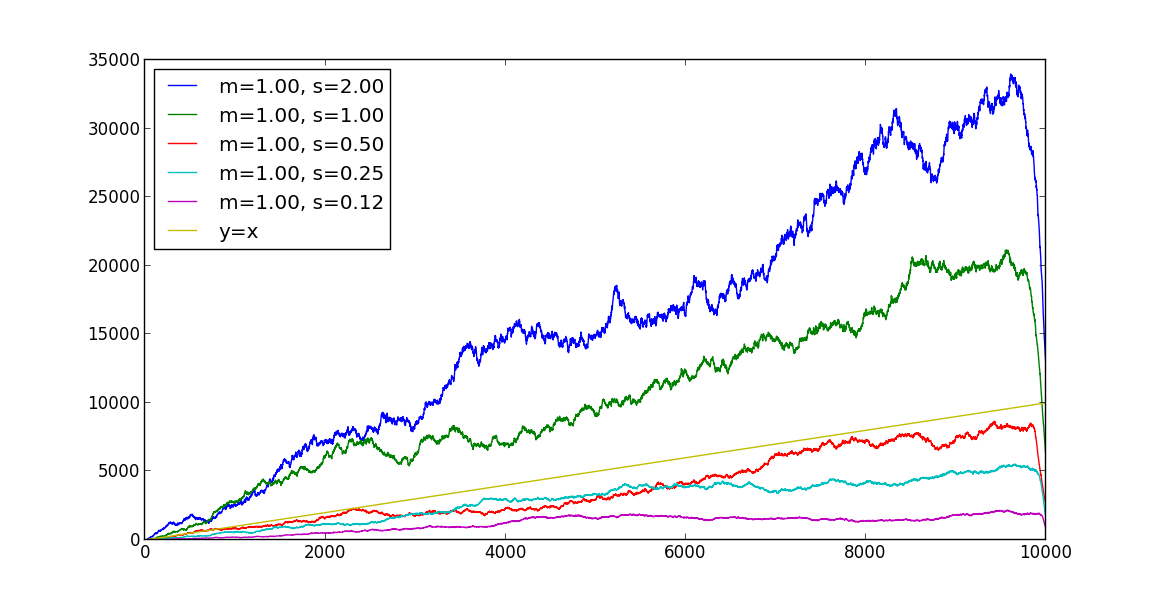
\includegraphics[scale=0.4]{figs/all.png}
  \caption{The evolution of $(n_{a} - n_{b})^{2}$ over time depending on the variance $\sigma$.}
  \label{fig:brownian}
  \end{figure}

Brownian motion $\langle (n_{a} - n_{b})^{2} \rangle \sim t$, where $n_{a}$ and $n_{b}$ are the number of messages in the channels $a$ and $b$ respectively, and $t$ is time. The average for $(n_{a} - n_{b})$ is taken for 30 experiments. Dependencies close to the Brownian motion $\bar{\Delta l^2} = 2Dt$ take place with the mass diffusivity $D$ as shown in the table below (Коэффициент определен на глаз. По хорошему надо аппроксимировать до прямой: брать среднее от углов наклона для прямых, проведенных через каждую точку). (Probably need to show that the dependency is linear with some statistical criteria like $\chi^{2}$ ?)
  \begin{tabular}{c|c|c|c}
  $m$ & $\sigma$ & $2D$ & $D$\\
  \hline
  $1$ & $2$ & $4$ & $2$\\
  \hline
  $1$ & $1$ & $2$ & $1$\\
  \hline
  $1$ & $0.5$ & $1$ & $0.5$\\
  \hline
  $1$ & $0.25$ & $0.5$ & $0.25$\\
  \hline
  $1$ & $0.125$ & $0.125$ & $0.125$\\ 
  \end{tabular}

Нужно пересчитать эксперимент для $m \neq 1$. Получается что-то похожее на $D = \frac{\sigma}{m^{2}}$. See \ref{fig:brownian}.

It would be good to find $D$ analiticaly!

  \section{The channel length dependent throughtput formula}
The general case probability matrix is in Table \ref{tbl:zip2_prob_mat}.

In our example we assume that both input channels are the same, i.e. the interarrival time in both channels is distributed according to the same law $Gamma(k,\theta,t_t)$. Then, the probability to see 1 message in the channel $a$ and see no messages in the channel $b$ over the time $t_t$ $P_a = P_b = p(1-p)$, where $p = Gamma(k,\theta,t_t)$ is the probability to see 1 message in a channel over time $t_t$.

$P_{ab} = P_{ba} = \frac{p^2}{2}$ is the probability to see 1 message in the channel $a$ and 1 message in the channel $b$, and $b$ after $a$. the probability to see no messages in the channels over time $t_t$ $P_n = (1-p)^2$.


\begin{sidewaystable}
  %\centering
  % make the table fit onto the page
  \scriptsize
  % stretch the rows in the table
  \def\arraystretch{2}
  \begin{tabular}{c|c|>{\centering\arraybackslash}p{2.1cm}|c|c|c|>{\centering\arraybackslash}p{2.1cm}|c|c|c}
  & $\mathbf{A_0 \: B_0 \: L_0}$ & $\mathbf{A_k \: B_0 \: L_0}$ & $\mathbf{A_{l-1} \: B_0 \: L_1}$ & $\mathbf{A_l \: B_0 \: L_0}$ & $\mathbf{A_l \: B_0 \: L_1}$ & $\mathbf{A_0 \: B_k \: L_0}$ & $\mathbf{A_0 \: B_{l-1} \: L_1}$ & $\mathbf{A_0 \: B_l \: L_0}$ & $\mathbf{A_0 \: B_l \: L_1}$\\
  \hline
  $\mathbf{A_0 \: B_0 \: L_0}$ & $P_n+P_{ab}+P_{ba}$ & $P_a \: (k=1)$ & 0 & 0 & 0 & $P_b \: (k=1)$ & 0 & 0 & 0\\
  \hline
  $\mathbf{A_j \: B_0 \: L_0}$ & $P_b \: (j=1)$ & $P_a \: (k-j=1)$, \par $P_b \: (j-k=1)$, \par $P_n+P_{ab}+P_{ba} \: (j=k)$ & 0 & $P_a \: (l-j=1)$ & 0 & 0 & 0 & 0 & 0\\
  \hline
  $\mathbf{A_{l-1} \: B_0 \: L_1}$ & $P_b \: (l=2)$ & $P_b \: (k=l-2)$, \par $P_n+P_{ab}+P_{ba} \: (k=l-1)$ & $P_n$ & $P_a$ & 0 & 0 & 0 & 0 & 0\\
  \hline
  $\mathbf{A_l \: B_0 \: L_0}$ & 0 & $P_b \: (l-k=1)$ & $P_{ab}$ & $P_n+P_{ba}$ & $P_a$ & 0 & 0 & 0 & 0\\
  \hline
  $\mathbf{A_l \: B_0 \: L_1}$ & 0 & $P_b \: (l-k=1)$ & $P_{ab}$ & $P_{ba}$ & $P_n+P_a$ & 0 & 0 & 0 & 0\\
  \hline
  $\mathbf{A_0 \: B_j \: L_0}$ & $P_a \: (j=1)$ & 0 & 0 & 0 & 0 & $P_b \: (k-j=1)$, \par $P_a \: (j-k=1)$, \par $P_n+P_{ab}+P_{ba} \: (j=k)$ & 0 & $P_b \: (l-j=1)$ & 0\\
  \hline
  $\mathbf{A_0 \: B_{l-1} \: L_1}$ & $P_a \: (l=2)$ & 0 & 0 & 0 & 0 & $P_a \: (k=l-2)$ \par $P_n+P_{ab}+P_{ba} \: (k=l-1)$ & $P_n$ & $P_b$ & 0\\
  \hline
  $\mathbf{A_0 \: B_l \: L_0}$ & 0 & 0 & 0 & 0 & 0 & $P_a \: (l-k=1)$ & $P_{ba}$ & $P_n+P_{ab}$ & $P_b$\\
  \hline
  $\mathbf{A_0 \: B_l \: L_1}$ & 0 & 0 & 0 & 0 & 0 & $P_a \: (l-k=1)$ & $P_{ba}$ & $P_{ab}$ & $P_n+P_b$\\
  \end{tabular}
  \caption{The general case probability matrix for the zip2 synchroniser}
  \label{tbl:zip2_prob_mat}
\end{sidewaystable}


Let $x_{i,j,k}$ denote the steady-state probability of the state $A_i \: B_j \: L_k$. Then $x = (x_{i,j,k})$ is the vector of statedy-state probabilities. Expanding $xP = x$ for $l>2$, we get the following system of linear equations:

\begin{equation}
\begin{cases}
    x_{0,0,0} = (P_n+P_{ab}+P_{ba}) \cdot x_{0,0,0} + P_b \cdot x_{1,0,0} + P_a \cdot x_{0,1,0},\\
    x_{k,0,0} = P_a \cdot x_{k-1,0,0} + (P_n+P_{ab}+P_{ba}) \cdot x_{k,0,0} + P_b \cdot x_{k+1,0,0}, \; k < l-2,\\
    x_{l-2,0,0} = P_a \cdot x_{l-3,0,0} + (P_n+P_{ab}+P_{ba}) \cdot x_{l-2,0,0} + P_b \cdot x_{l-1,0,0} + P_b \cdot x_{l-1,0,1},\\
    x_{l-1,0,0} = P_a \cdot x_{l-2,0,0} + (P_n+P_{ab}+P_{ba}) \cdot x_{l-1,0,0} + (P_{ab}+P_{ba}) \cdot x_{l-1,0,1} + P_b \cdot x_{l,0,0} + P_b \cdot x_{l,0,1},\\
    x_{l-1,0,1} = P_n \cdot x_{l-1,0,1} + P_{ab} \cdot x_{l,0,0} + P_{ab} \cdot x_{l,0,1},\\
    x_{l,0,0} = P_a \cdot x_{l-1,0,0} + P_a \cdot x_{l-1,0,1} + (P_n+P_{ba}) \cdot x_{l,0,0} + P_{ba} \cdot x_{l,0,1},\\
    x_{l,0,1} = P_a \cdot x_{l,0,0} + (P_n+P_a) \cdot x_{l,0,1},\\
    \cdots\\
    x_{0,0,0} + \sum_{k=1}^{l} x_{k,0,0} + x_{l-1,0,1} + x_{l,0,1} + \sum_{k=1}^{l} x_{0,k,0} + x_{0,l-1,1} + x_{0,l,1} = 1
\end{cases}
\end{equation}

Knowing that distributions in channels have the same parameters, we conclude that $x_{k,0,0} = x_{0,k,0}, \; 1<k<l$ and $x_{l-1,0,1}=x_{0,l-1,1}, \; x_{l,0,1}=x_{0,l,1}$. Then we find 

\end{appendices}

\end{document}
